\section{Results and further studies}
\label{sec:candcresults}
The distribution of the dilepton invariant mass in the central and forward signal regions are shown in Figure~\ref{fig:resultsCC}. The resulting event yields are compared to the expectation from SM backgrounds in Table~\ref{tab:METresults2012}. A maximum likelihood fit is performed in each region to find the best estimator for the for the difference of expected and observed yield. The significances of deviations of this difference from zero are evaluated using the profile likelihood ratio of the signal and signal+background hypothesis~\cite{HiggsTool1}. In general, the observed data is in agreement with the background estimation within about one standard deviation, except for the low-mass region in the central dilepton selection. Here the observed yield exceeds the expectation by $109^{+48}_{-49}$ events. The size of this excess corresponds to a significance of 2.2~$\sigma$.  
\begin{figure}[htbp]
\centering
\begin{minipage}[t]{0.49\textwidth}
  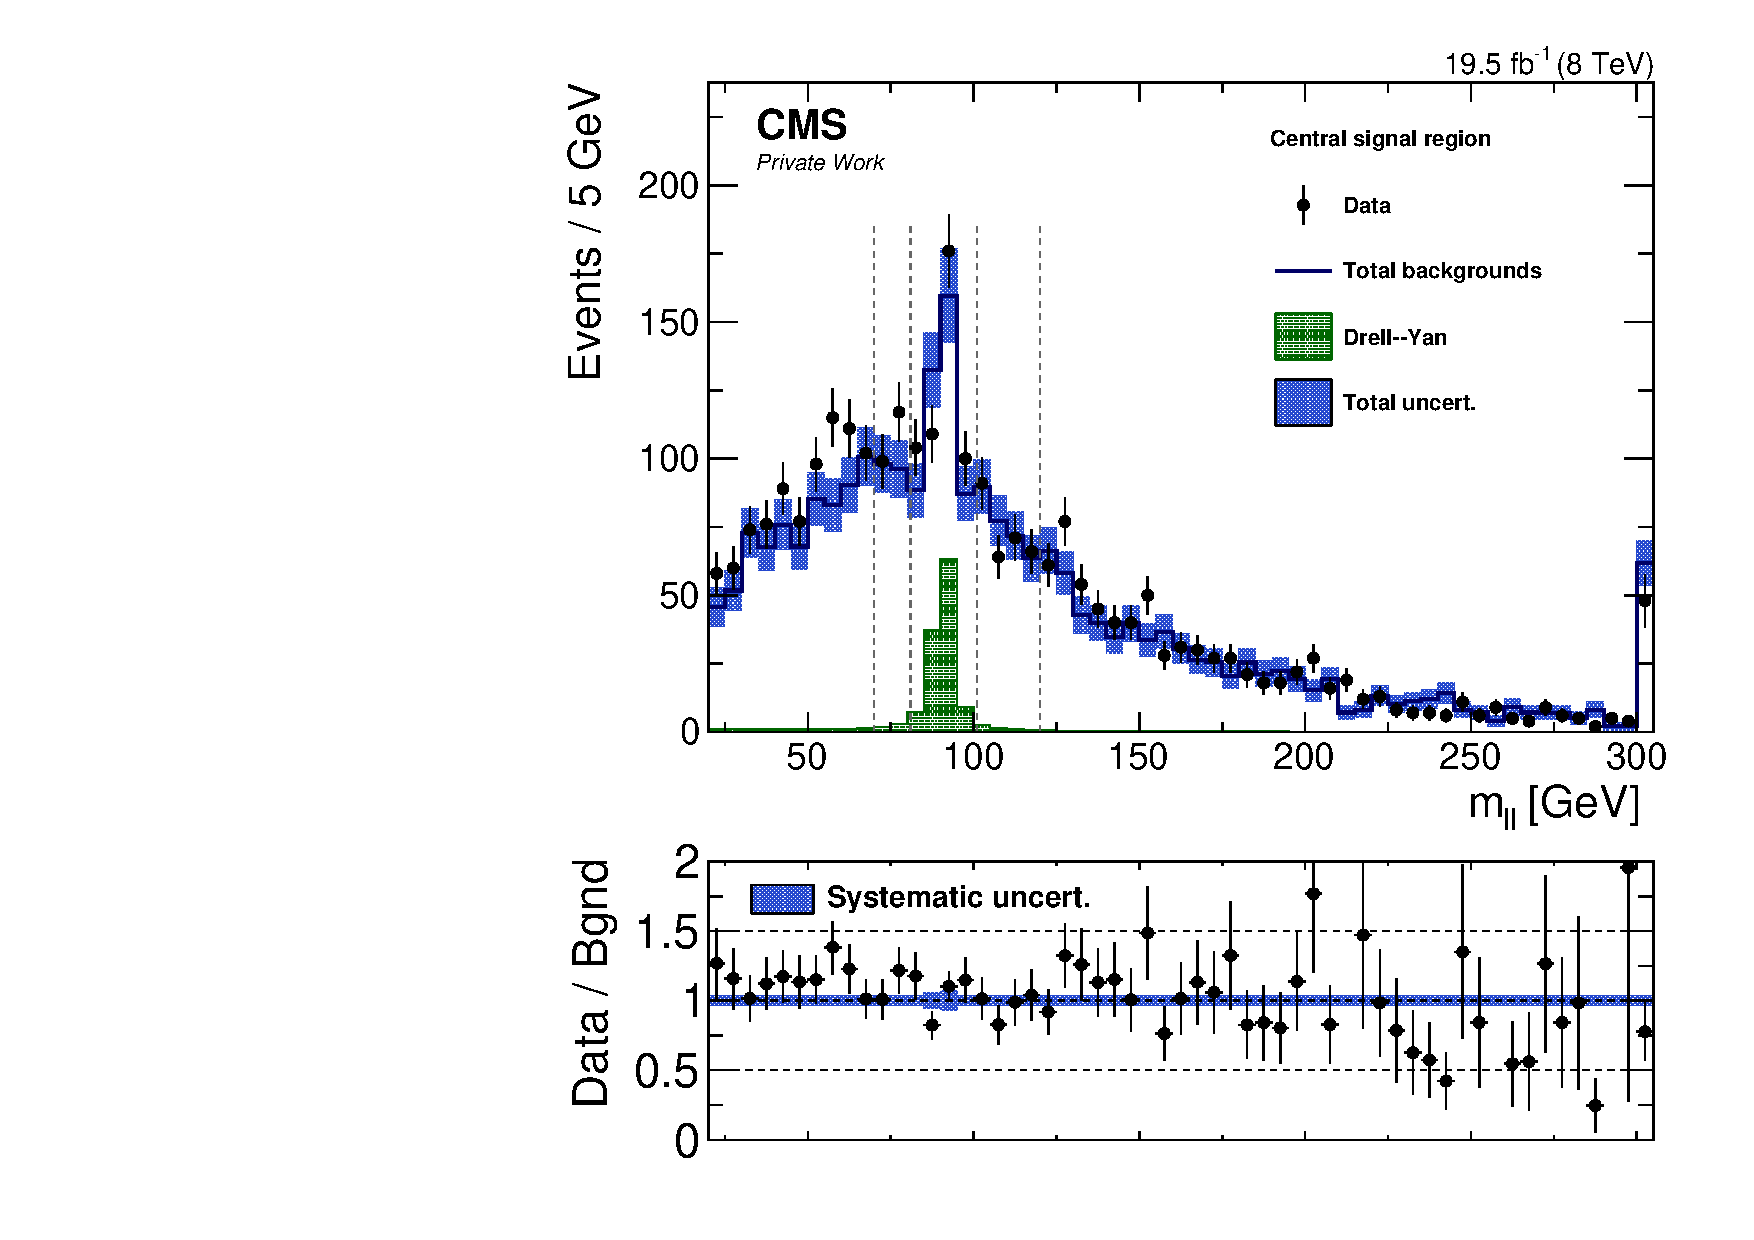
\includegraphics[width=\textwidth]{plots/results/mllResult_SignalCentral_Full2012_SF.pdf}
\end{minipage}
\begin{minipage}[t]{0.49\textwidth}
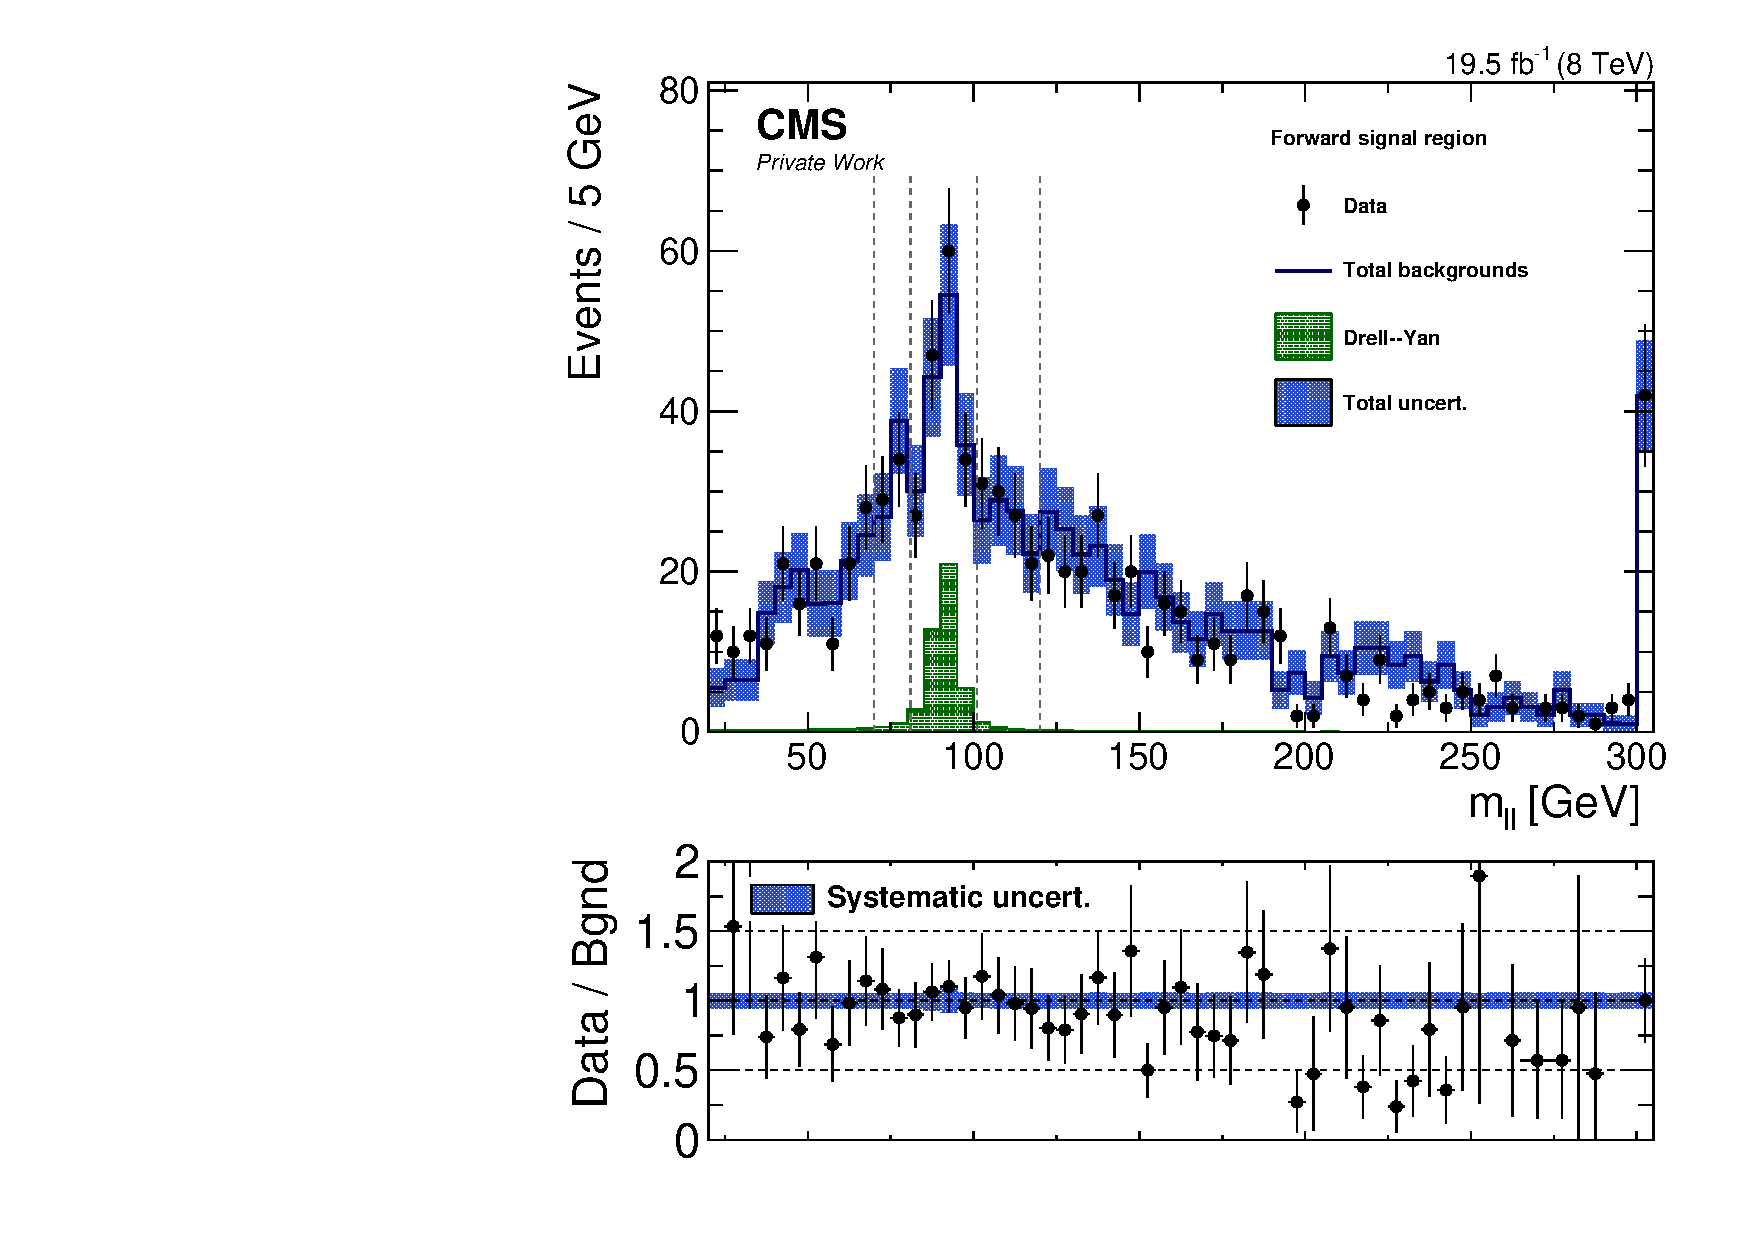
\includegraphics[width=\textwidth]{plots/results/mllResult_SignalForward_Full2012_SF.pdf}
\end{minipage}

\caption{Distribution of \mll in the signal region for the central (left) and forward (right) dilepton selection. The data is shown as black dots, while the total background prediction from data is shown as a blue histogram. The blue error bars indicate the combined statistical and systematic background uncertainty in each bin. The contribution from backgrounds containing a Z boson is shown as a green histogram. The dashed lines indicates the boundaries of the three mass bins. Beneath the plot the ratio of data to the background prediction is shown. The error bars include the statistical uncertainties of data and background, while the blue band indicates the systematic uncertainties on the background. }
\label{fig:resultsCC}
\end{figure} 


\begin{table}[btp]
 \renewcommand{\arraystretch}{1.3}
 \setlength{\belowcaptionskip}{6pt}
 \scriptsize
 \centering
 \caption{Results of the counting experiment in the six signal regions.
     The statistical and systematic uncertainties are added in quadrature, except for the flavor-symmetric backgrounds. The presented differences between the observed and estimated yields are obtained with a maximum likelihood fit (see text).    Low-mass refers to $20\GeV < \mll < 70$\GeV, on-\Z to  $81\GeV < \mll < 101$\GeV, and high-mass to $\mll > 120$\GeV.
     }
  \label{tab:METresults2012}
  \begin{tabular}{l| cc | cc | cc}

    							& \multicolumn{2}{c}{low-mass} & \multicolumn{2}{c}{on-\Z} & \multicolumn{2}{c}{high-mass} \\ 

    \hline
                                &  Central        & Forward  &  Central  & Forward   &  Central        & Forward \\ 

    \hline
        Observed       &  865                   & 154              &  494            &  176       &   849           &   381    \\

    \hline
        Flav.-sym.    & $746\pm27\pm26$        & $144\pm12\pm7$  &  $368\pm19\pm13$ & $137\pm11\pm7$ & $789\pm28\pm28$ & $411\pm20\pm21$ \\

            Drell--Yan          & $8.6\pm2.7$            & $2.6\pm0.8$      & $119\pm21$ & $43\pm9$ & $2.7\pm0.8$ & $1.2\pm0.4$ \\

    \hline
            Total est.          & $755\pm38$            & $147\pm14$      & $488\pm31$ & $180\pm16$ & $792\pm39$ & $413\pm30$ \\

    \hline
         Obs. - est.  & $109\pm48$      & $7\pm19$ & $6\pm38 $ & $-5\pm21$ & $57\pm50$ & $-32\pm37 $ \\ 

    \hline
   Significance      & 2.2~$\sigma$    &  0.4~$\sigma$  & 0.1~$\sigma$ & $<$0.1~$\sigma$ & 1.1~$\sigma$ & $<$0.1~$\sigma$ \\ 


  \end{tabular}
\end{table}



In the Tables~\ref{tab:METresults2012MM} and~\ref{tab:METresults2012EE}, the results are shown separately for \EE and \MM events. As expected from the fact that \rmue is larger than one, the yields in the \MM channel are slightly larger than in the \EE channel. For the flavour-symmetry backgrounds, and therefore also for the total background estimates and the difference of observation and estimation, the yields in the \EE and \MM channels to not exactly add up to those in the combined SF channel. \fixme{Reference explenation once written} 

\begin{table}[hbtp]
 \renewcommand{\arraystretch}{1.3}
 \setlength{\belowcaptionskip}{6pt}
 \scriptsize
 \centering
 \caption{Results of the counting experiment for \EE events only.
     The statistical and systematic uncertainties are added in quadrature, except for the flavor-symmetric backgrounds. The presented differences between the observed and estimated yields are obtained with a maximum likelihood fit (see text).    Low-mass refers to $20 < \mll < 70$\GeV, on-\Z to  $81 < \mll < 101$\GeV, and high-mass to $\mll > 120$\GeV.
     }
  \label{tab:METresults2012EE}
  \begin{tabular}{l| cc | cc | cc}

    							& \multicolumn{2}{c}{low-mass} & \multicolumn{2}{c}{on-\Z} & \multicolumn{2}{c}{high-mass} \\ 

    \hline
                                &  Central        & Forward  &  Central  & Forward   &  Central        & Forward \\ 

    \hline
        Observed       &  389                   & 53              &  232            &  86       &   401           &   195    \\

    \hline
        Flav.-sym.    & $337\pm12\pm19$        & $61\pm5\pm6$  &  $166\pm8\pm9$ & $58\pm5\pm5$ & $357\pm12\pm21$ & $175\pm8\pm17$ \\

            Drell--Yan          & $4.3\pm1.3$            & $1.2\pm0.4$      & $62\pm11$ & $21\pm5$ & $1.5\pm0.5$ & $0.7\pm0.2$ \\

    \hline
            Total est.          & $342\pm23$            & $62\pm8$      & $229\pm17$ & $79\pm9$ & $358\pm24$ & $175\pm19$ \\

    \hline
         Obs. - est.  & $47\pm25$      & $-10\pm9$ & $3\pm21 $ & $6\pm12$ & $42\pm26$ & $19\pm18 $ \\ 

    \hline
   Significance      & 1.9~$\sigma$    &  $<$0.1~$\sigma$  & 0.1~$\sigma$ & 0.5~$\sigma$ & 1.7~$\sigma$ & 1.1~$\sigma$ \\ 


  \end{tabular}
\end{table}





\begin{table}[hbtp]
 \renewcommand{\arraystretch}{1.3}
 \setlength{\belowcaptionskip}{6pt}
 \scriptsize
 \centering
 \caption{Results of the counting experiment for \MM events only.
     The statistical and systematic uncertainties are added in quadrature, except for the flavor-symmetric backgrounds.
     Low-mass refers to $20 < \mll < 70$\GeV, on-\Z to  $81 < \mll < 101$\GeV and high-mass to $\mll > 120$\GeV.
     }
  \label{tab:METresults2012MM}
  \begin{tabular}{l| cc | cc | cc}

    							& \multicolumn{2}{c}{low-mass} & \multicolumn{2}{c}{on-\Z} & \multicolumn{2}{c}{high-mass} \\ 

    \hline
                                &  Central        & Forward  &  Central  & Forward   &  Central        & Forward \\ 

    \hline
        Observed       &  476                   & 101              &  262            &  90       &   448           &   186    \\

    \hline
        Flavor-symmetric    & $405\pm14\pm21$        & $79\pm6\pm6$  &  $200\pm10\pm10$ & $74\pm6\pm6$ & $428\pm15\pm23$ & $224\pm11\pm19$ \\

            Drell--Yan          & $4.4\pm1.4$            & $1.6\pm0.6$      & $58\pm10$ & $25\pm6$ & $1.2\pm0.4$ & $0.7\pm0.2$ \\

    \hline
            Total estimated          & $409\pm26$            & $80\pm9$      & $258\pm18$ & $100\pm11$ & $429\pm27$ & $225\pm22$ \\

    \hline
         Observed - estimated  & $67^{+29}_{-29}$      & $20^{+13}_{-13}$ & $3^{+22}_{-23} $ & $-11^{+13}_{-13}$ & $19^{+29}_{-29}$ & $-40^{+21}_{-21} $ \\ 

    \hline
   Significance      & 2.3~$\sigma$    &  1.6~$\sigma$  & 0.2~$\sigma$ & $<$0.1~$\sigma$ & 0.6~$\sigma$ & $<$0.1~$\sigma$ \\ 


  \end{tabular}
\end{table}







\begin{figure}[htbp]
\centering
\begin{minipage}[t]{0.49\textwidth}
  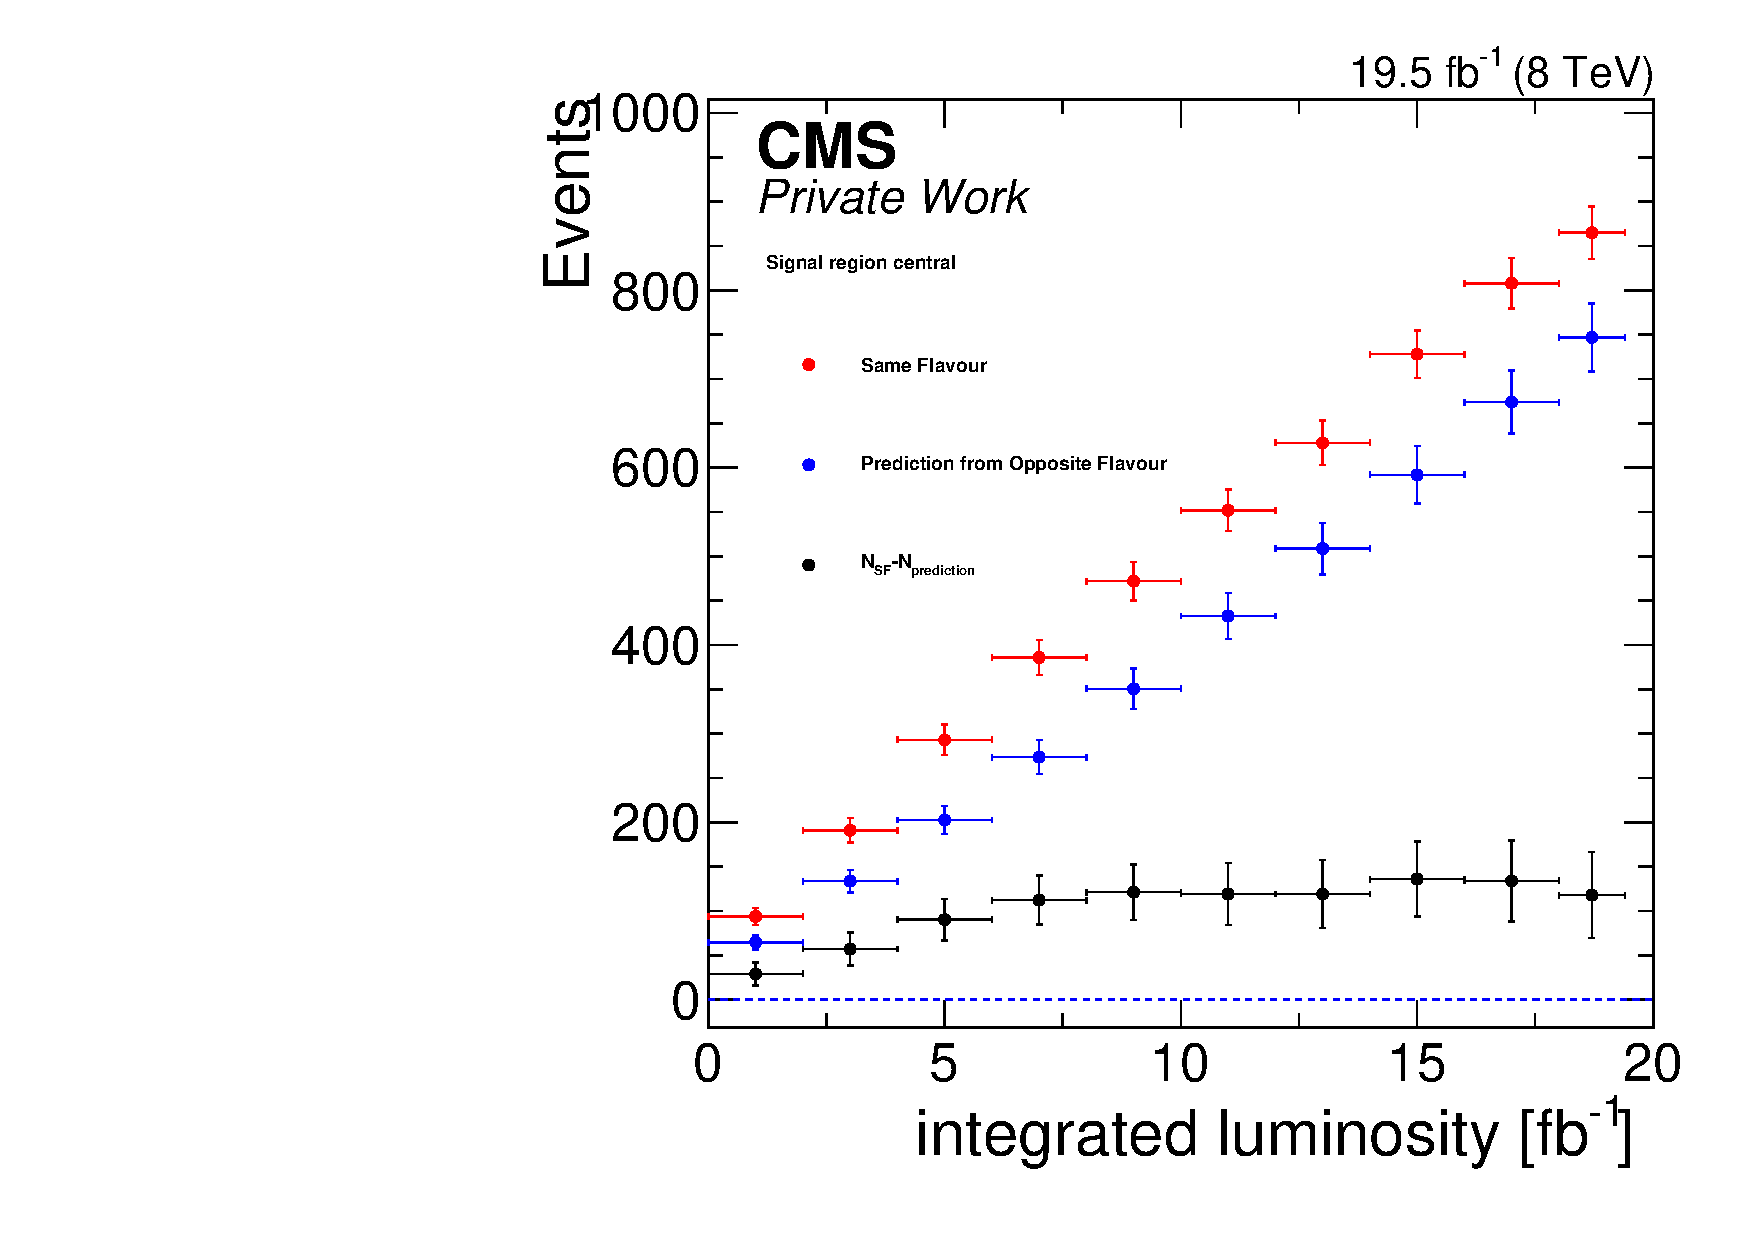
\includegraphics[width=\textwidth]{plots/results/YieldvsLumi_SignalCentral_Mll_edgeMassFull2012.pdf}
\end{minipage}
\begin{minipage}[t]{0.49\textwidth}
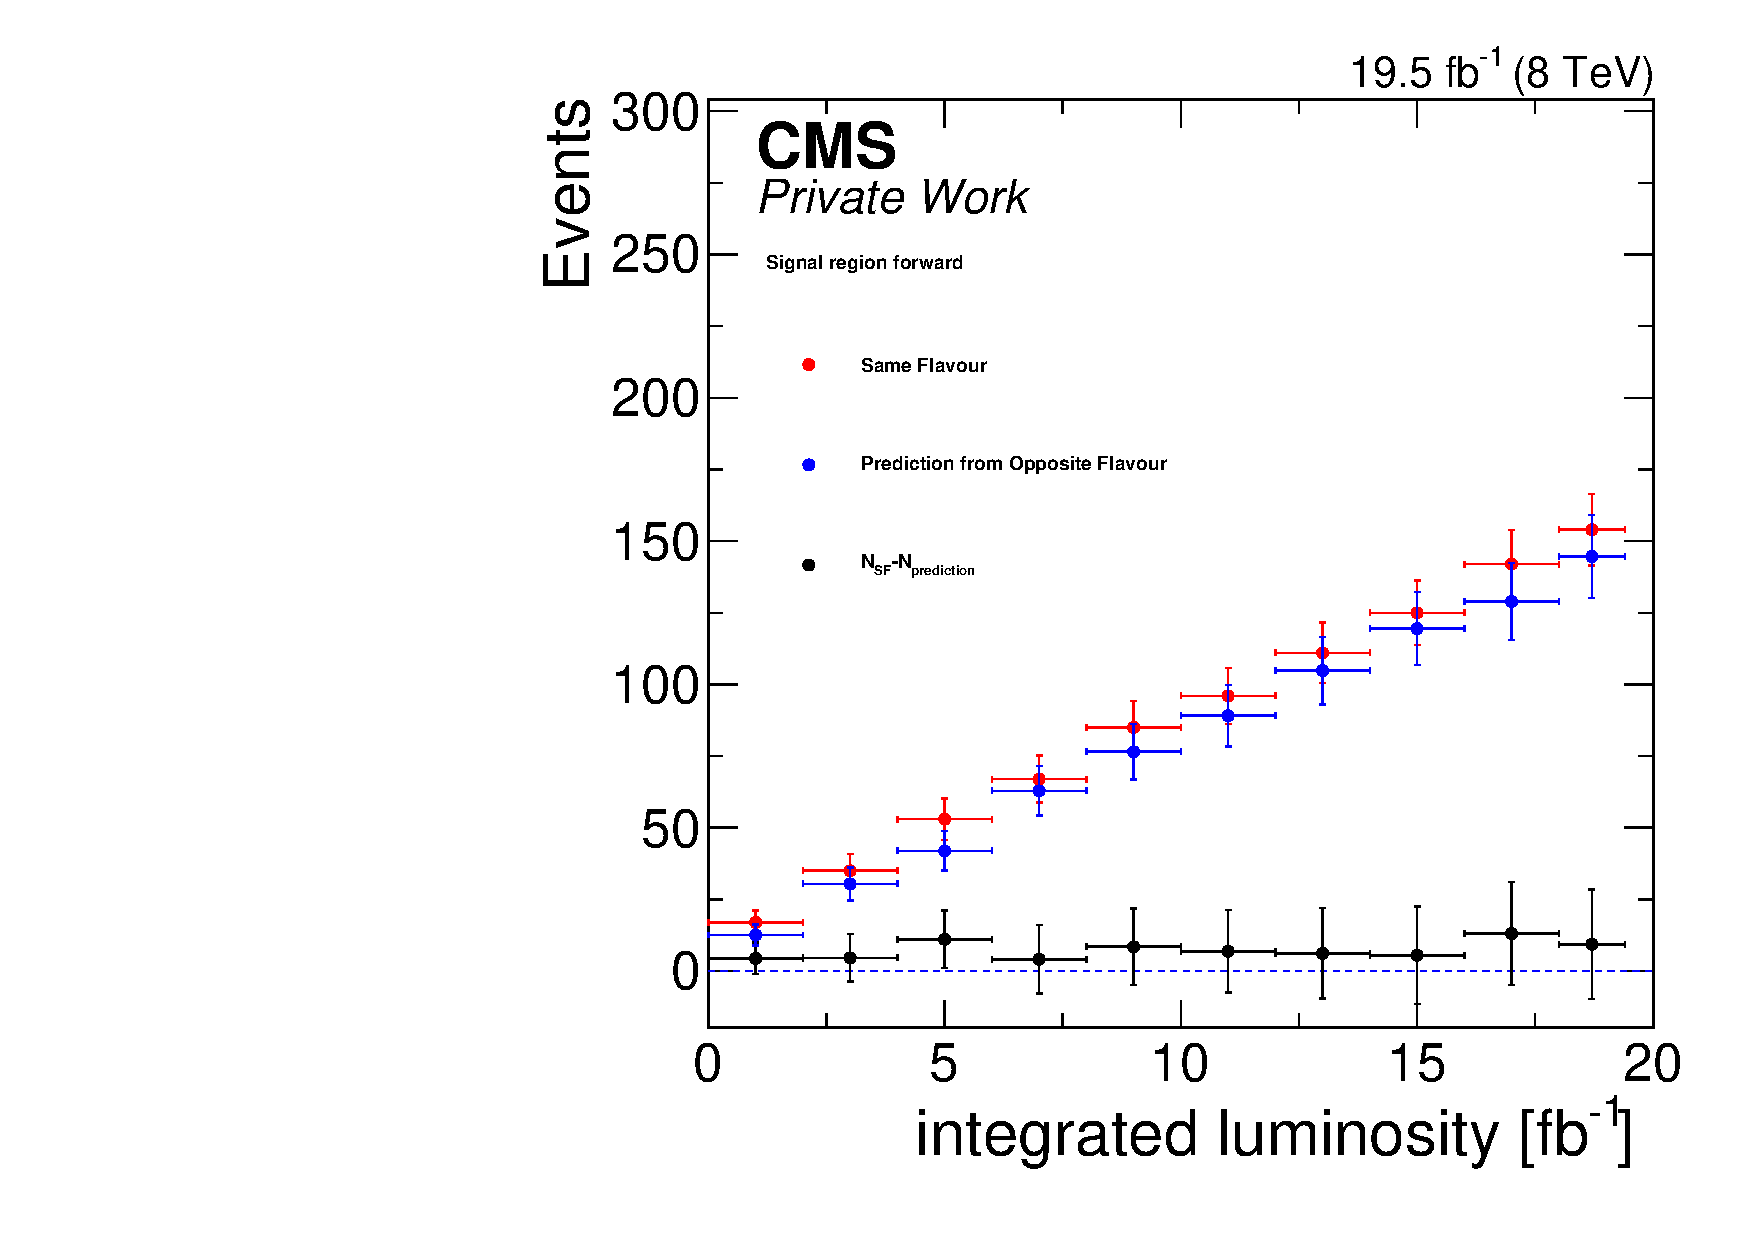
\includegraphics[width=\textwidth]{plots/results/YieldvsLumi_SignalForward_Mll_edgeMassFull2012.pdf}
\end{minipage}

\caption{Distribution of \mll in the signal region for the central (left) and forward (right) dilepton selection. The data is shown as black dots, while the total background prediction from data is shown as a blue histogram. The blue error bars indicate the combined statistical and systematic background uncertainty in each bin. The contribution from backgrounds containing a Z boson is shown as a green histogram. The dashed lines indicates the boundaries of the three mass bins. Beneath the plot the ratio of data to the background prediction is shown. The error bars include the statistical uncertainties of data and background, while the blue band indicates the systematic uncertainties on the background. }
\label{fig:timeDependece}
\end{figure}





\begin{table}[hbtp]
 \renewcommand{\arraystretch}{1.3}
 \setlength{\belowcaptionskip}{6pt}
 \centering
 \caption{Results of the counting experiment in the low-mass central signal region for different variations of the event selection. The observed event yield in SF events is compared with the combined estimate from flavour-symmetric and Drell--Yan backgrounds. The estimate for the Drell--Yan backgrounds is obtained by extrapolating the event yield in the on-Z signal region after subtraction of flavour-symmetric backgrounds to the low-mass region using the \Routin factor.}
  \label{tab:CountingCrosschecks}
  \begin{tabular}{l|c|c|c|c}
                                &  SF        & Flavour-symmetric  &  Drell--Yan  & Observed - Estimates \\ 

    \hline
    \hline
 & \multicolumn{4}{c}{b-tagging}\\ 
\hline 
        no b-tags       &  202                   & 188.5$\pm$15.4              &  7.1$\pm$2.5            &  6.3$\pm$21.1 \\
        $\geq$ 1 b-tags       &  663                   & 558.4$\pm$31.0              &  1.9$\pm$0.7            &  102.7$\pm$40.3 \\
\hline 
 & \multicolumn{4}{c}{lepton \pt requirement} \\ 
\hline 
        \pt > 20(10)\GeV       &  1474                   & 1290.2$\pm$58.6              &  11.4$\pm$4.1            &  172.5$\pm$70.1 \\
        \pt > 30(10)\GeV       &  1262                   & 1114.8$\pm$52.1              &  11.3$\pm$4.1            &  135.9$\pm$63.2 \\
        \pt > 30(20)\GeV       &  761                   & 674.0$\pm$35.5              &  9.0$\pm$3.3            &  78.0$\pm$45.1 \\
        \pt > 30\GeV       &  296                   & 275.7$\pm$19.4              &  6.5$\pm$2.3            &  13.8$\pm$26.0 \\
\hline 
 & \multicolumn{4}{c}{tight lepton isolation} \\ 
\hline 
        rel. isolation < 0.05       &  572                   & 491.5$\pm$28.4              &  7.1$\pm$2.6            &  73.3$\pm$37.2 \\
\hline 
 & \multicolumn{4}{c}{pileup} \\ 
\hline 
        $N_{\text{vtx}} <$ 13       &  332                   & 289.9$\pm$20.0              &  3.3$\pm$1.2            &  38.8$\pm$27.1 \\
        13 $\leq N_{\text{vtx}}$ < 17       &  242                   & 212.8$\pm$16.5              &  0.9$\pm$0.3            &  28.3$\pm$22.7 \\
        $N_{\text{vtx}} \geq$ 17       &  291                   & 244.2$\pm$18.0              &  4.8$\pm$1.7            &  41.9$\pm$24.8 \\
\hline 
 & \multicolumn{4}{c}{\MET reconstructions}\\
\hline 
        type I corrected PF \MET       &  1034                   & 923.3$\pm$45.0              &  9.4$\pm$3.4            &  101.3$\pm$55.4 \\
        track corrected \MET       &  850                   & 702.3$\pm$36.6              &  26.3$\pm$9.4            &  121.3$\pm$47.7 \\
        missing $H_{\mathrm{T}}$       &  1171                   & 942.5$\pm$45.7              &  50.8$\pm$18.1            &  177.6$\pm$59.9 \\
\hline 
 & \multicolumn{4}{c}{$H_{\mathrm{T}}$}\\
\hline 
        100\GeV $< H_{\mathrm{T}} < $ 300\GeV        &  455                   & 401.3$\pm$24.7              &  1.4$\pm$0.5            &  52.3$\pm$32.7 \\
        $H_{\mathrm{T}} > $ 300\GeV        &  410                   & 344.6$\pm$22.4              &  7.5$\pm$2.7            &  57.9$\pm$30.3 \\
\hline 


  \end{tabular}
\end{table}





\begin{figure}[htbp]
\centering
\begin{minipage}[t]{0.49\textwidth}
  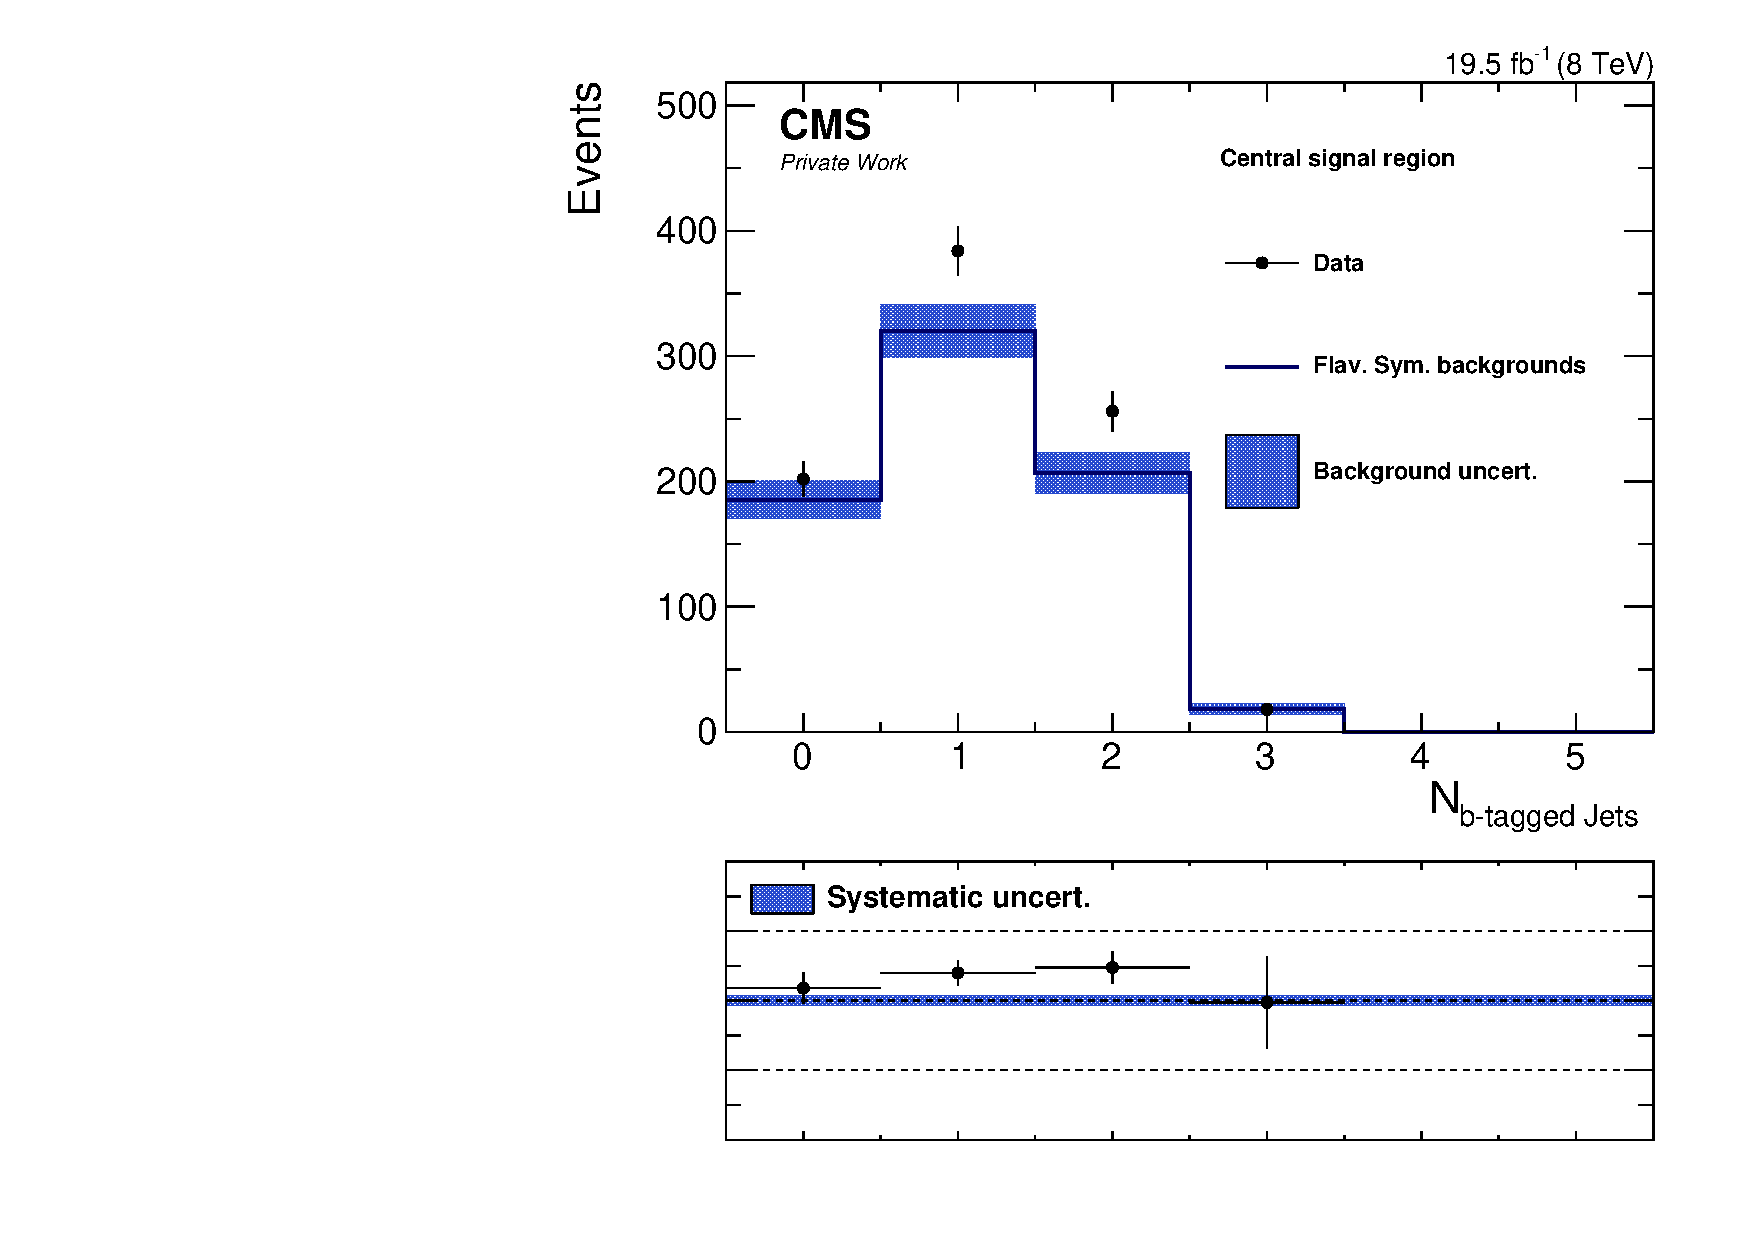
\includegraphics[width=\textwidth]{plots/results/rSFOFDependencies/rSFOFDependency_SignalCentral_NBJets_Full2012_SF_lowMass.pdf}
\end{minipage}
\begin{minipage}[t]{0.49\textwidth}
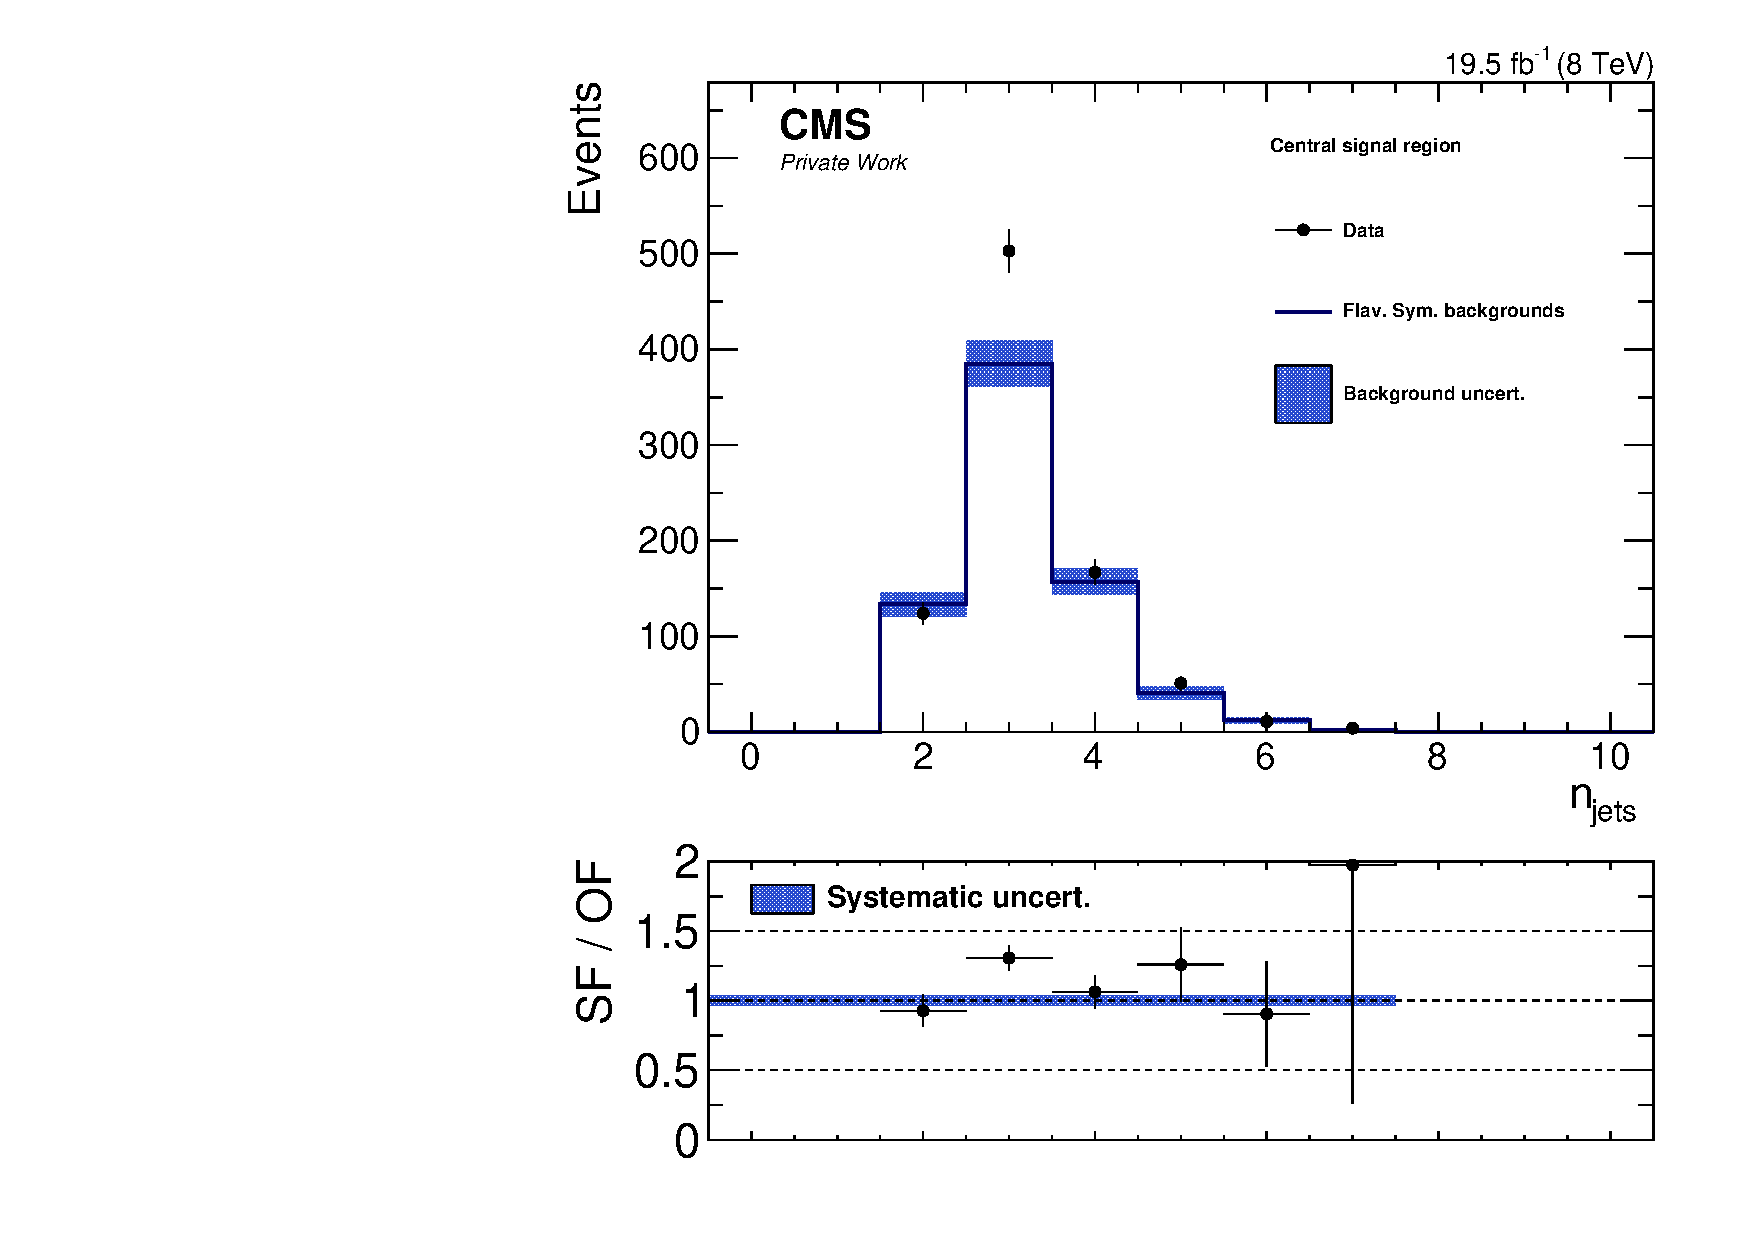
\includegraphics[width=\textwidth]{plots/results/rSFOFDependencies/rSFOFDependency_SignalCentral_NJets_Full2012_SF_lowMass.pdf}
\end{minipage}
\begin{minipage}[t]{0.49\textwidth}
  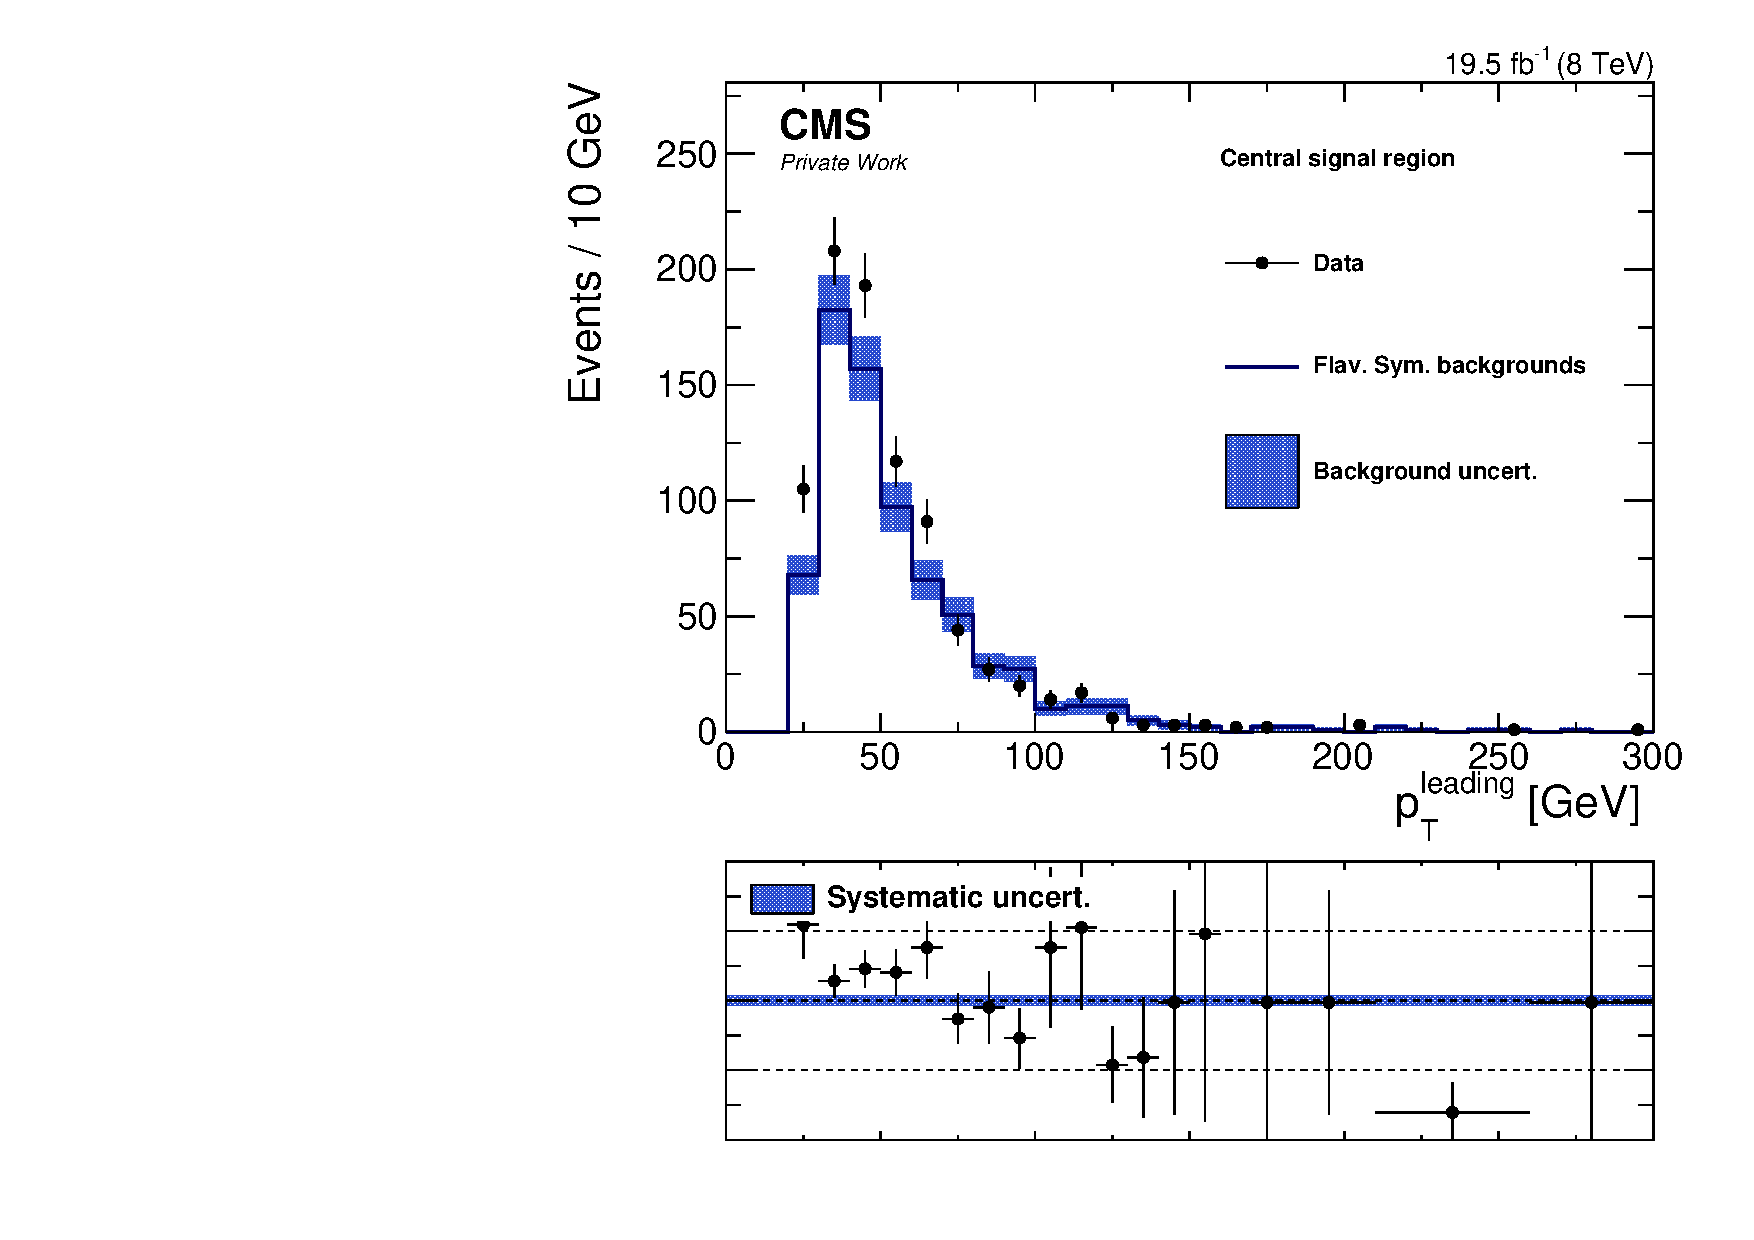
\includegraphics[width=\textwidth]{plots/results/rSFOFDependencies/rSFOFDependency_SignalCentral_LeadingPt_Full2012_SF_lowMass.pdf}
\end{minipage}
\begin{minipage}[t]{0.49\textwidth}
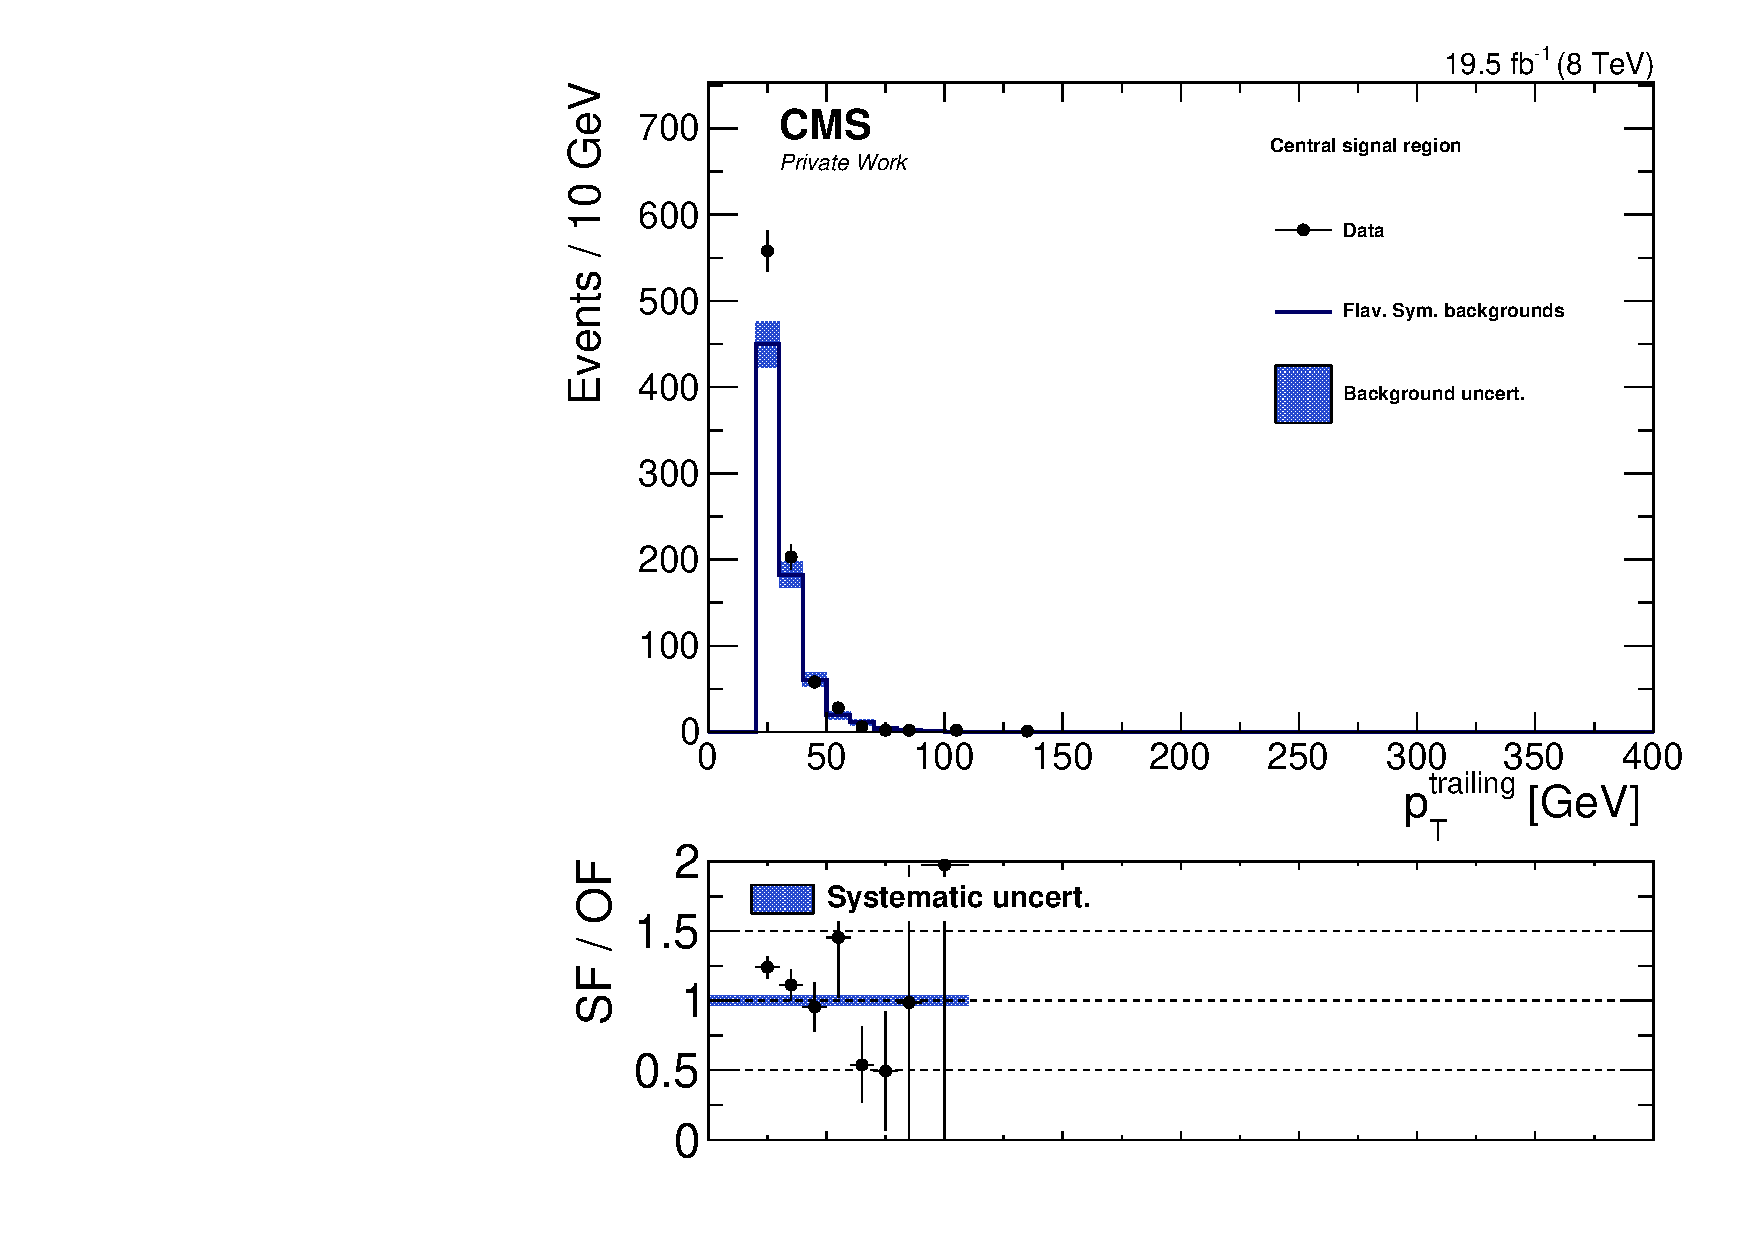
\includegraphics[width=\textwidth]{plots/results/rSFOFDependencies/rSFOFDependency_SignalCentral_TrailingPt_Full2012_SF_lowMass.pdf}
\end{minipage}
\begin{minipage}[t]{0.49\textwidth}
  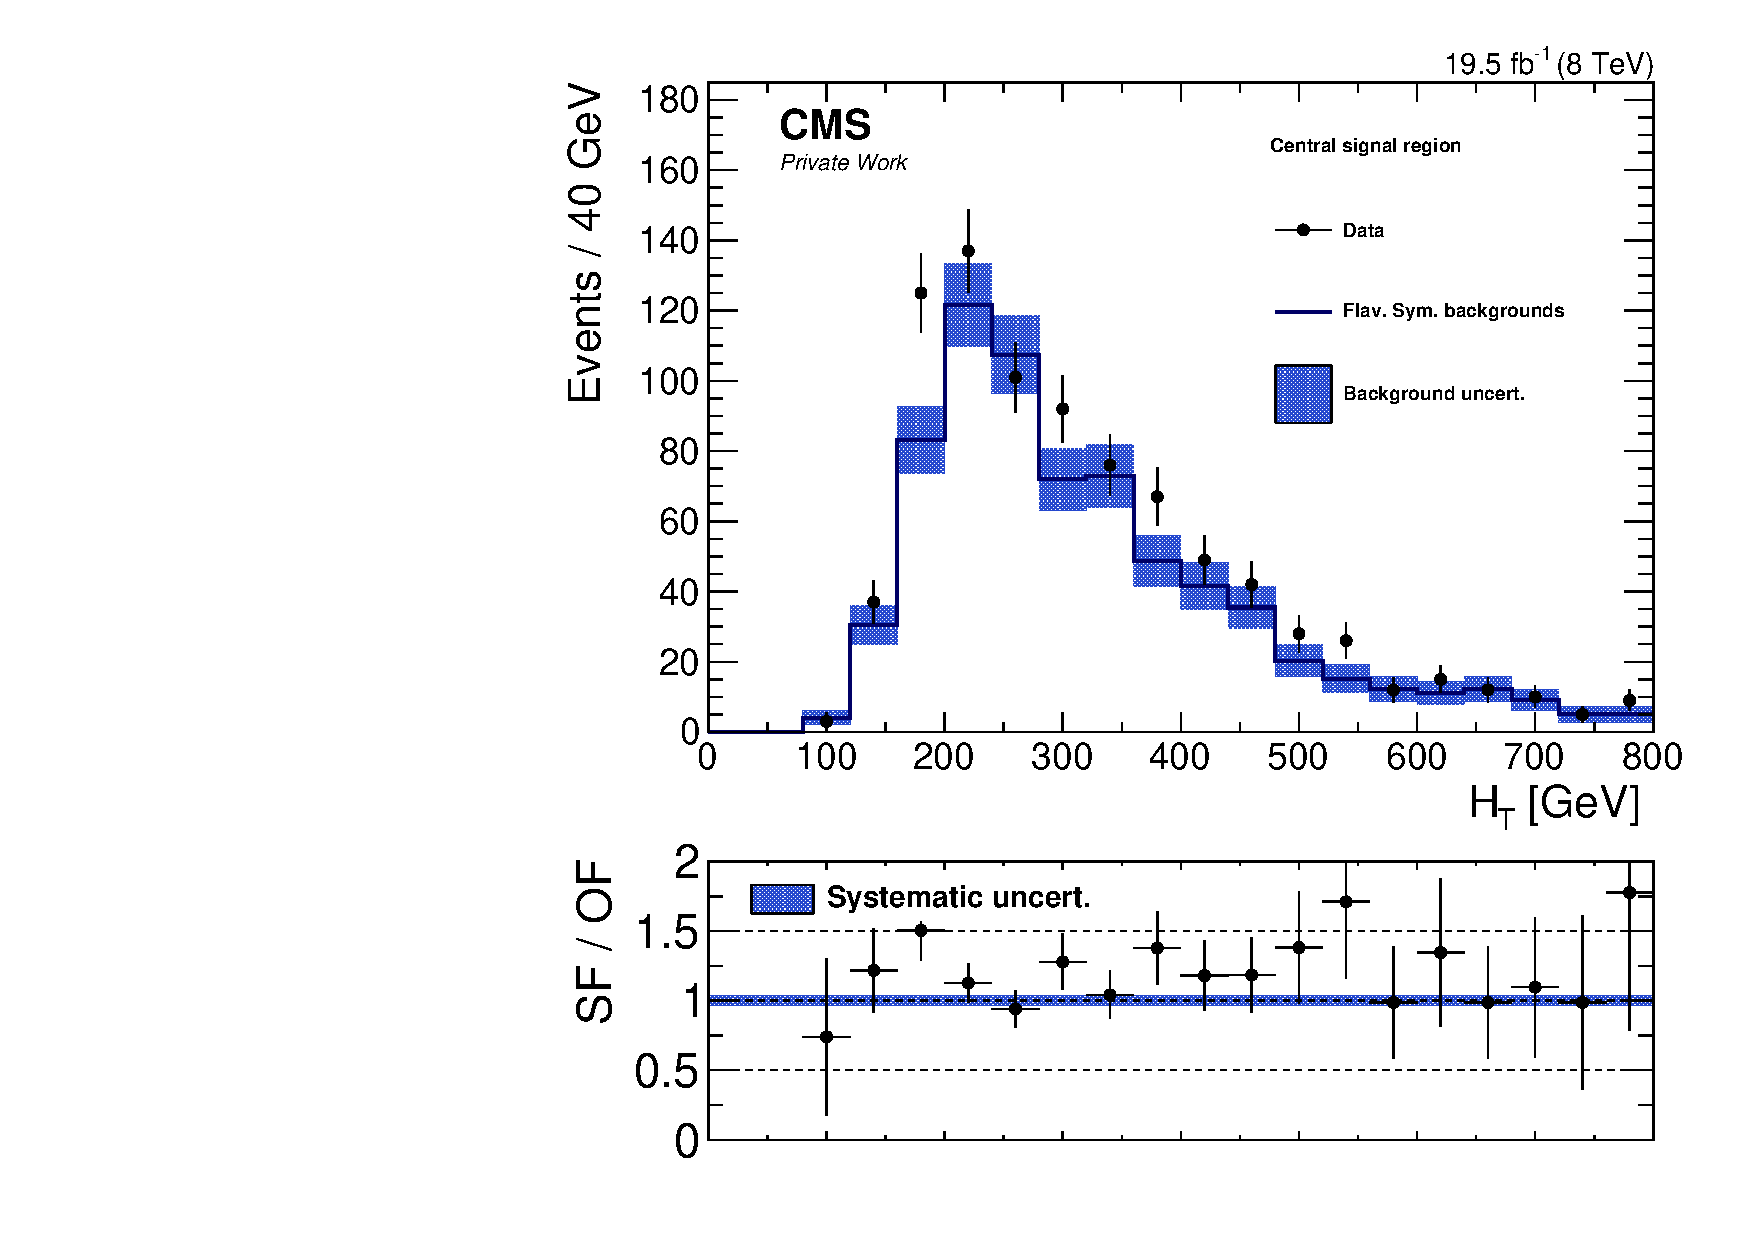
\includegraphics[width=\textwidth]{plots/results/rSFOFDependencies/rSFOFDependency_SignalCentral_HT_Full2012_SF_lowMass.pdf}
\end{minipage}
\begin{minipage}[t]{0.49\textwidth}
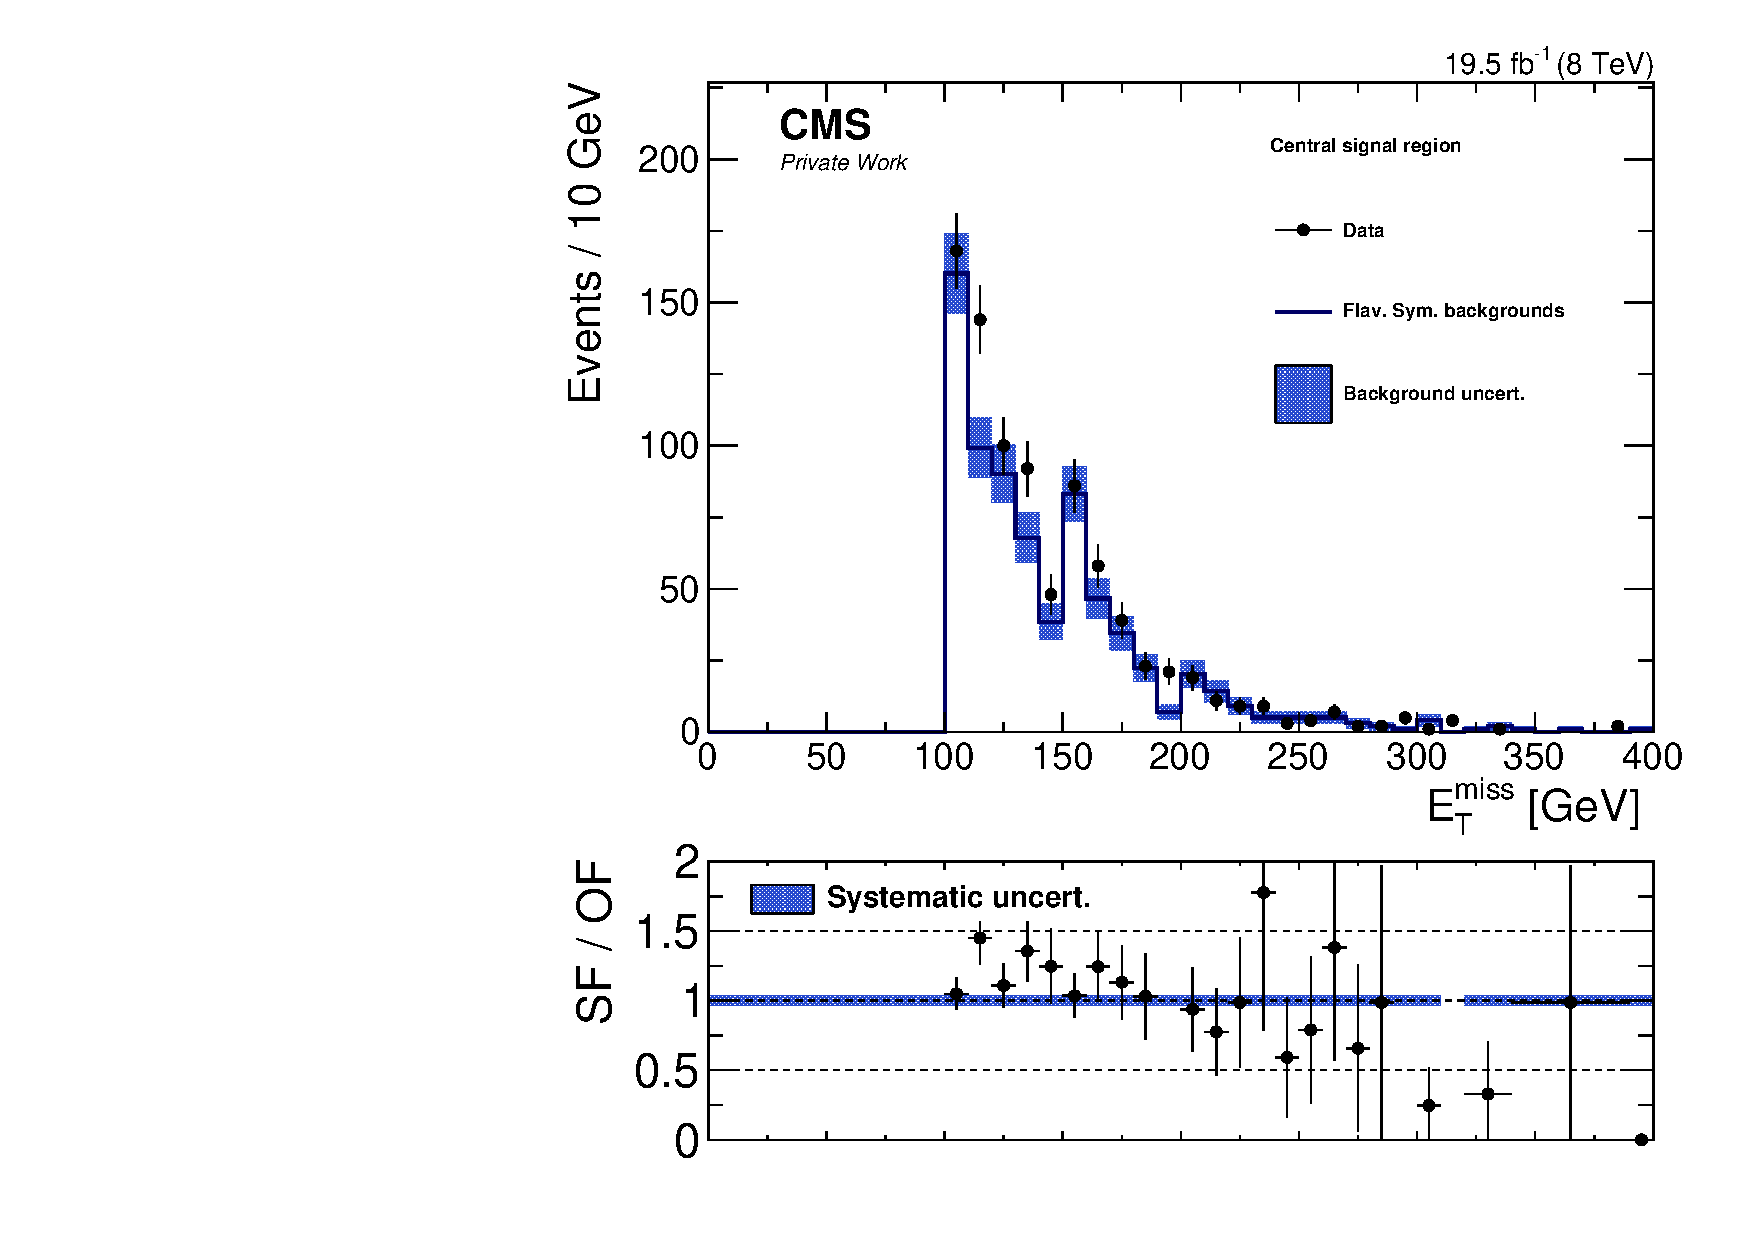
\includegraphics[width=\textwidth]{plots/results/rSFOFDependencies/rSFOFDependency_SignalCentral_MET_Full2012_SF_lowMass.pdf}
\end{minipage}
\caption{Distribution of \mll in the signal region for the central (left) and forward (right) dilepton selection. The data is shown as black dots, while the total background prediction from data is shown as a blue histogram. The blue error bars indicate the combined statistical and systematic background uncertainty in each bin. The contribution from backgrounds containing a Z boson is shown as a green histogram. The dashed lines indicates the boundaries of the three mass bins. Beneath the plot the ratio of data to the background prediction is shown. The error bars include the statistical uncertainties of data and background, while the blue band indicates the systematic uncertainties on the background. }
\label{fig:timeDependece}
\end{figure}


\section{Interpretation in simplified models}
The absence of a clear indication for the existence of SUSY in the results of the counting experiment presented in Section~\ref{sec:candcresults} constrains the validity of supersymmetric models. To quantify the impact these results have on the allowed parameter space, they are interpreted in specific signal scenarios. Here, the two simplified models discussed in Section~\ref{sec:models} are used. 

\subsubsection{Selection efficiencies}
The impact of branching fractions, detector acceptance, and selection efficiencies on the different signal points is shown in Figure~\ref{fig:sigEff} for the example of the central signal region for the fixed-edge (left) and slepton-edge (right) models. Because of the much larger branching fraction into lepton pairs in the case of the slepton-edge model, caused by the presence of the slepton in decay chain, the overall acceptance$\times$efficiency is an order of magnitude larger in this case. As the event kinematics vary depending on the sparticle masses, the efficiency strongly depends on the position of the signal point in the $m_{\sbottom}$-$m_{\secondchi}$ plane. In general, the efficiency is low along the diagonal, where little energy is available for the decay products. Another notable feature is a decrease in efficiency around \secondchi masses of about $\unit{225}{\giga\electronvolt}$ in the case of the slepton-edge model. This is caused by the gaps in the signal acceptance between the three invariant mass regions of the counting experiment. No such effect is visible for the fixed-edge case because the signal is concentrated in the low-mass region in this model.  
\begin{figure}[htbp]
\centering
\begin{minipage}[t]{0.49\textwidth}
  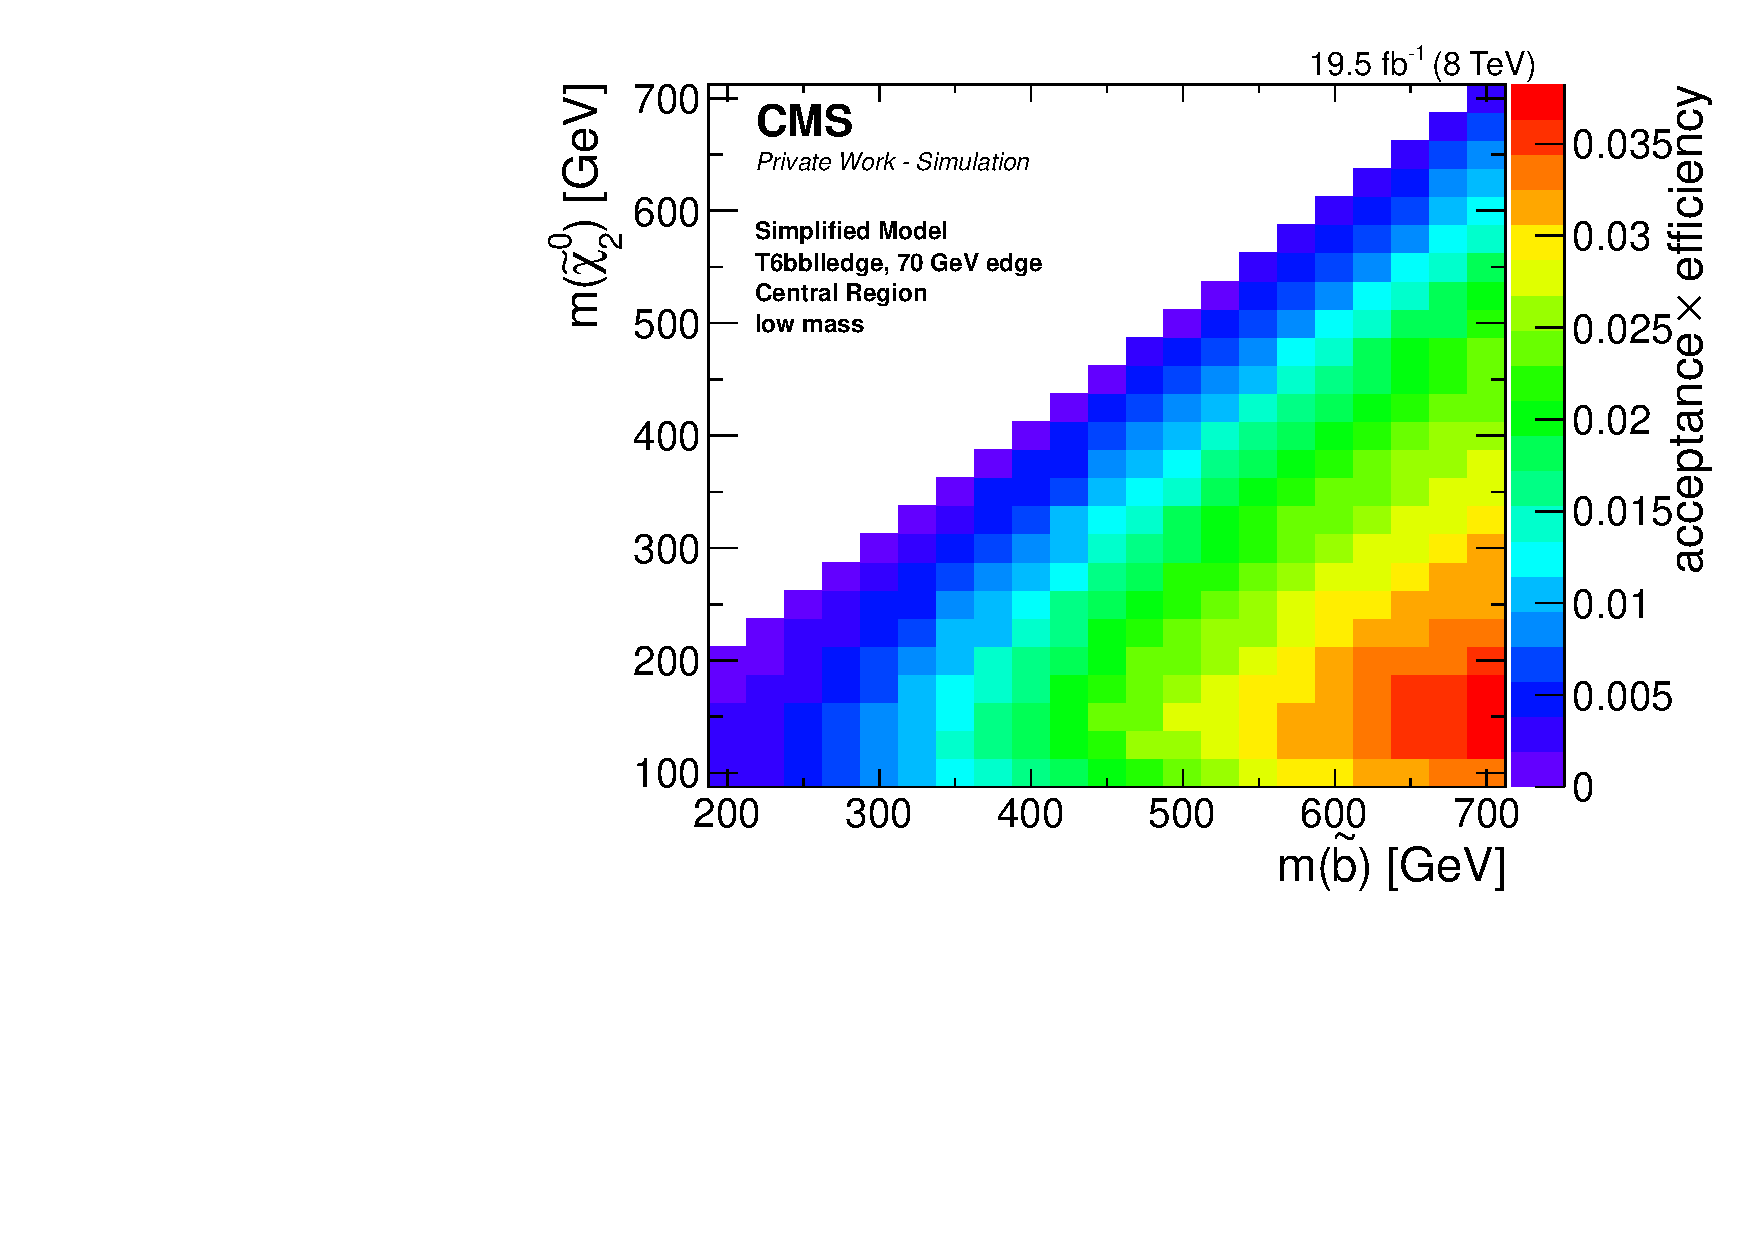
\includegraphics[width=\textwidth]{plots/limits/T6bblledge_70_GeV_Edge_Barrel_lowMll_signalEfficiency.pdf}
\end{minipage}
\begin{minipage}[t]{0.49\textwidth}
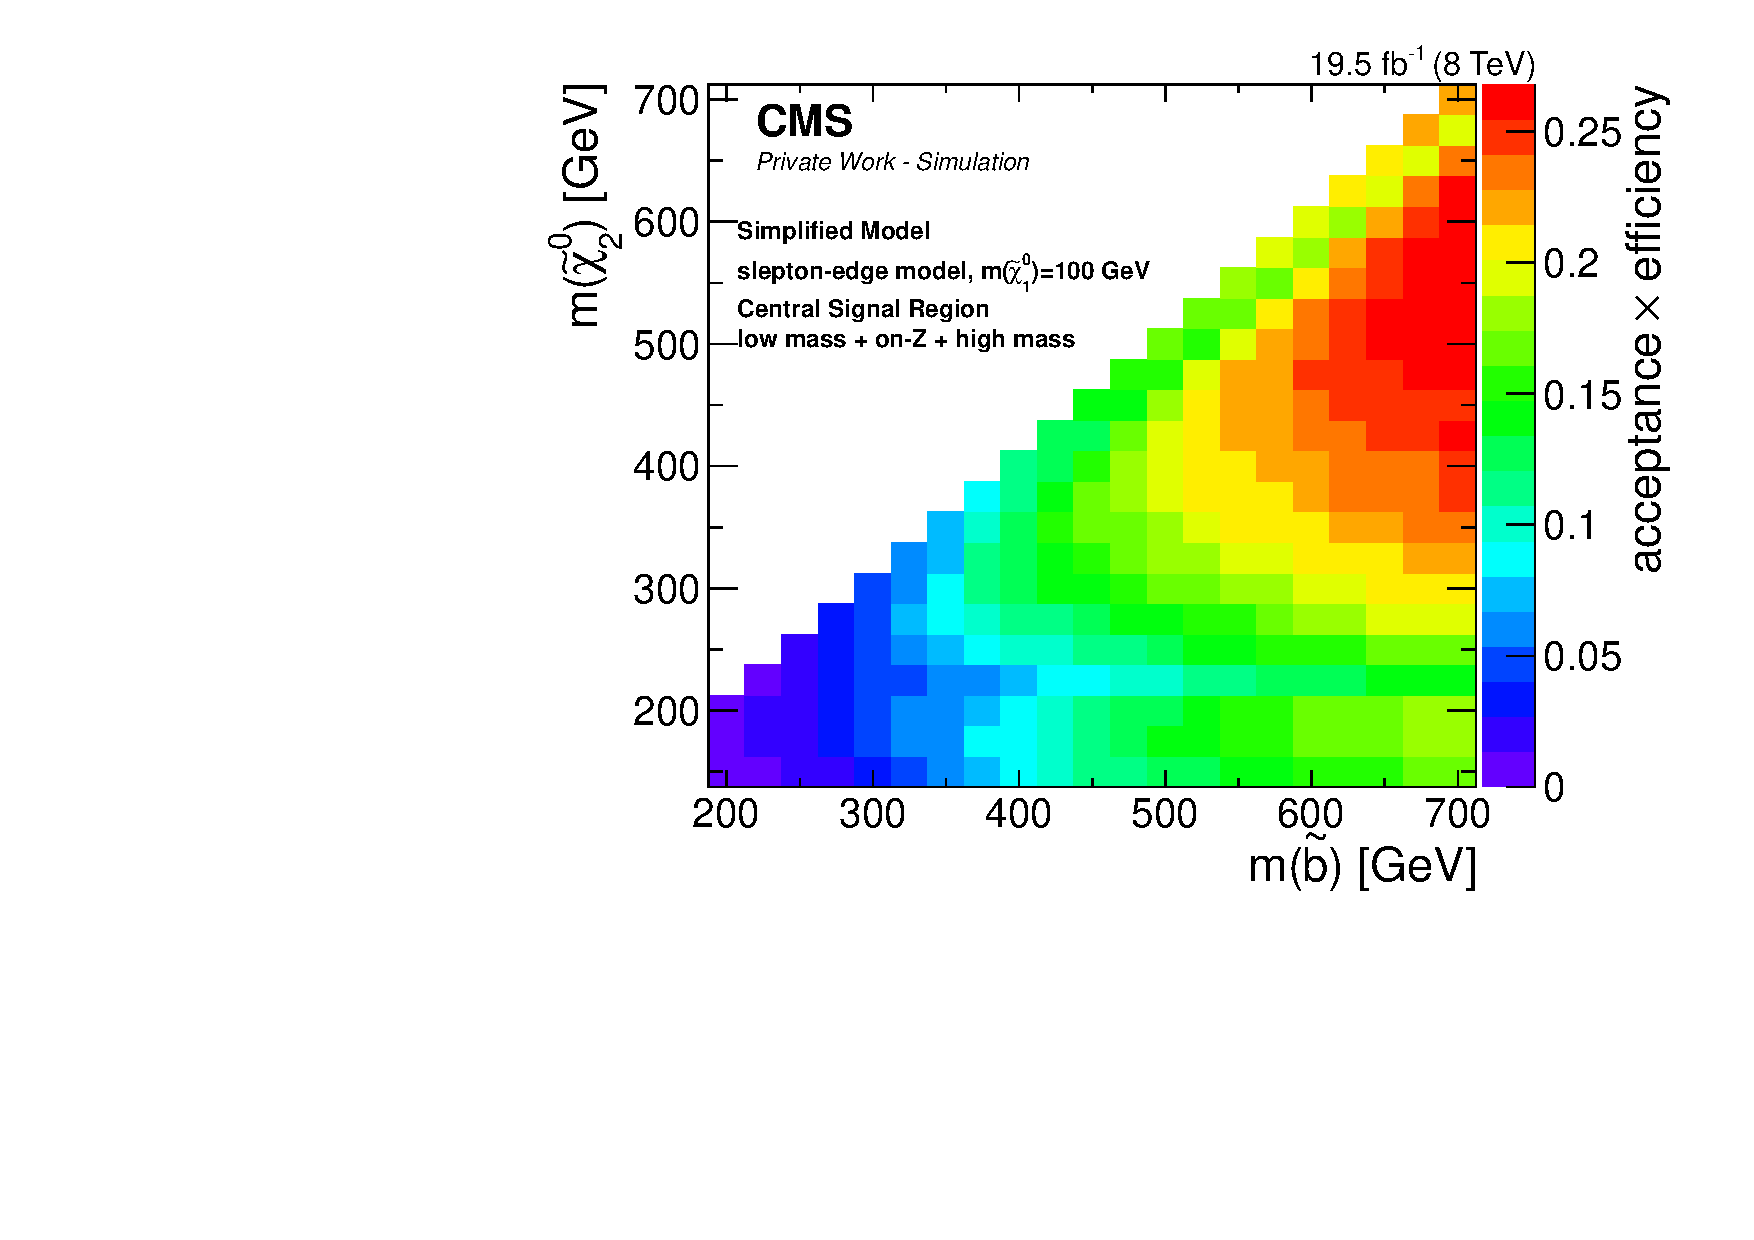
\includegraphics[width=\textwidth]{plots/limits/T6bbllslepton_m_n_1_100_Barrel_signalEfficiency_Reweighted.pdf}
\end{minipage}
\caption{Signal acceptance$\times$efficiency in the $m_{\sbottom}$-$m_{\secondchi}$ plane for the fixed-edge (left) and slepton-edge (right) model for the central signal region.}
\label{fig:sigEff}
\end{figure}
\subsubsection{Systematic uncertainties}
A variety of systematic uncertainties in the signal modelling have to taken into account. The integrated luminosity is measured with a precision of 2.6\%~\cite{CMS-PAS-LUM-13-001}. Variations of the parton distribution functions (PDF) according to the PDF4LHC recommendations~\cite{Alekhin:2011sk,Botje:2011sn,Ball:2012cx,Martin:2009iq,Lai:2010vv} result in an uncertainty of 0--6\% in the signal acceptance. Uncertainties related to lepton efficiencies are of the size of 1\% per lepton. Furthermore, the corrections of the lepton efficiency differences between fast and full detector simulation amount to another 1\% per lepton. The dilepton trigger efficiencies are measured with a precision of 5\%, as described in Section~\ref{sec:triggerEffs}. Uncertainties on the muon momentum scale have negligible impact on the signal acceptance, whereas the uncertainty in the electron energy scale is 0.6\% for central and 1.5\% for forward leptons. Jet energy scale uncertainties~\cite{1748-0221-6-11-P11002} result in an uncertainty in the signal yield of 0--8\%. The uncertainties in the modeling of the objects in the events are propagated to the \MET measurements, resulting in an uncertainty in the signal acceptance of 0--8\%. Here the contributions from the jet energy scale uncertainties are dominant. The events are corrected for difference between observed data and the modelling of initial-state-radiation (ISR) in Madgraph~\cite{Chatrchyan:2013xna} Uncertainties in these corrections are propagated to the event selection and result in an uncertainty of 0--14\% in the signal yield.
The uncertainty associated with pileup reweighting is evaluated by shifting the inelastic cross section by $\pm5\%$, resulting in an uncertainty on the signal acceptance of about 1\%. The uncertainties are summarised in Table~\ref{tab:sysUncerts}.

\begin{table}
\begin{center}
\caption{Summary of systematic uncertainties on the signal efficiency.}
\label{tab:sysUncerts}
\begin{tabular}{l|c}
Uncertainty source & Impact on signal yield [\%]\\ \hline 
Luminosity & 2.6 \\
PDFs on acceptance & 0--6 \\ 
Lepton identification/isolation & 2\\
Fast simulation lepton identification/isolation & 2 \\
Dilepton trigger & 5 \\
Lepton energy scale & 0--5  \\
\MET & 0--8  \\
Jet energy scale/resolution & 0--8  \\
ISR modeling & 0--14 \\
Additional interactions & 1 \\
%\multicolumn{2}{c}{Theoretical Uncertainties}\\
%\hline
%Fact./Renorm. Scale and PDFs& 14-18   \\
\end{tabular}
\end{center}
\end{table}
The combined systematic uncertainties are shown in Figure~\ref{fig:sys}. For the most part of the $m_{\sbottom}$-$m_{\secondchi}$ plane it ranges from 5-7\%. However, close to the diagonal this increases, caused by a larger impact of JES and ISR uncertainties. This is due to the overall lower jet \pt in this region, increasing the probability for threshold effects around the jet \pt requirement of $\unit{40}{\giga\electronvolt}$. The largest uncertainties are observed for both low masses of the \sbottom and \secondchi, exceeding 20\% for the fixed-edge model and   reaching 15\% for the slepton-edge model.
\begin{figure}[htbp]
\centering
\begin{minipage}[t]{0.49\textwidth}
  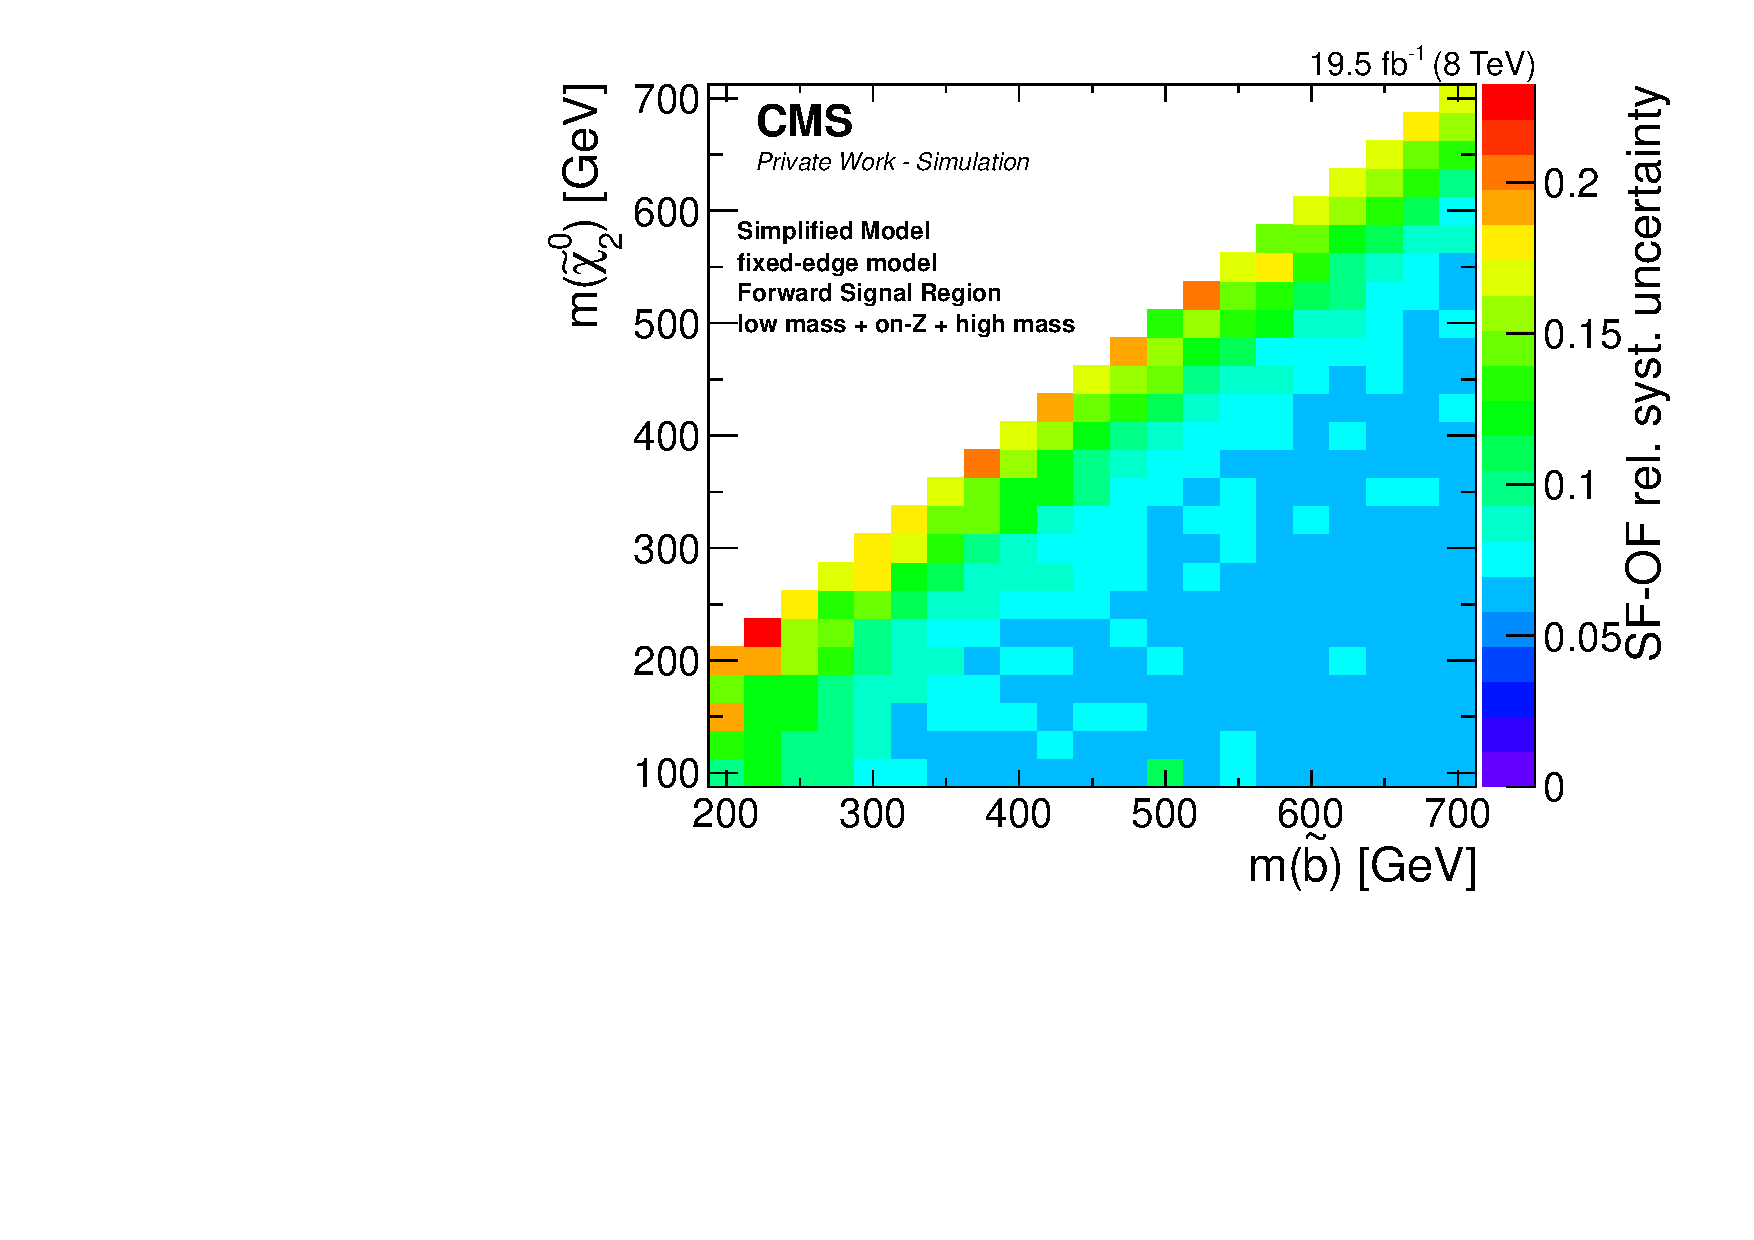
\includegraphics[width=\textwidth]{plots/limits/T6bblledge_70_GeV_Edge_Endcap_syst_err.pdf}
\end{minipage}
\begin{minipage}[t]{0.49\textwidth}
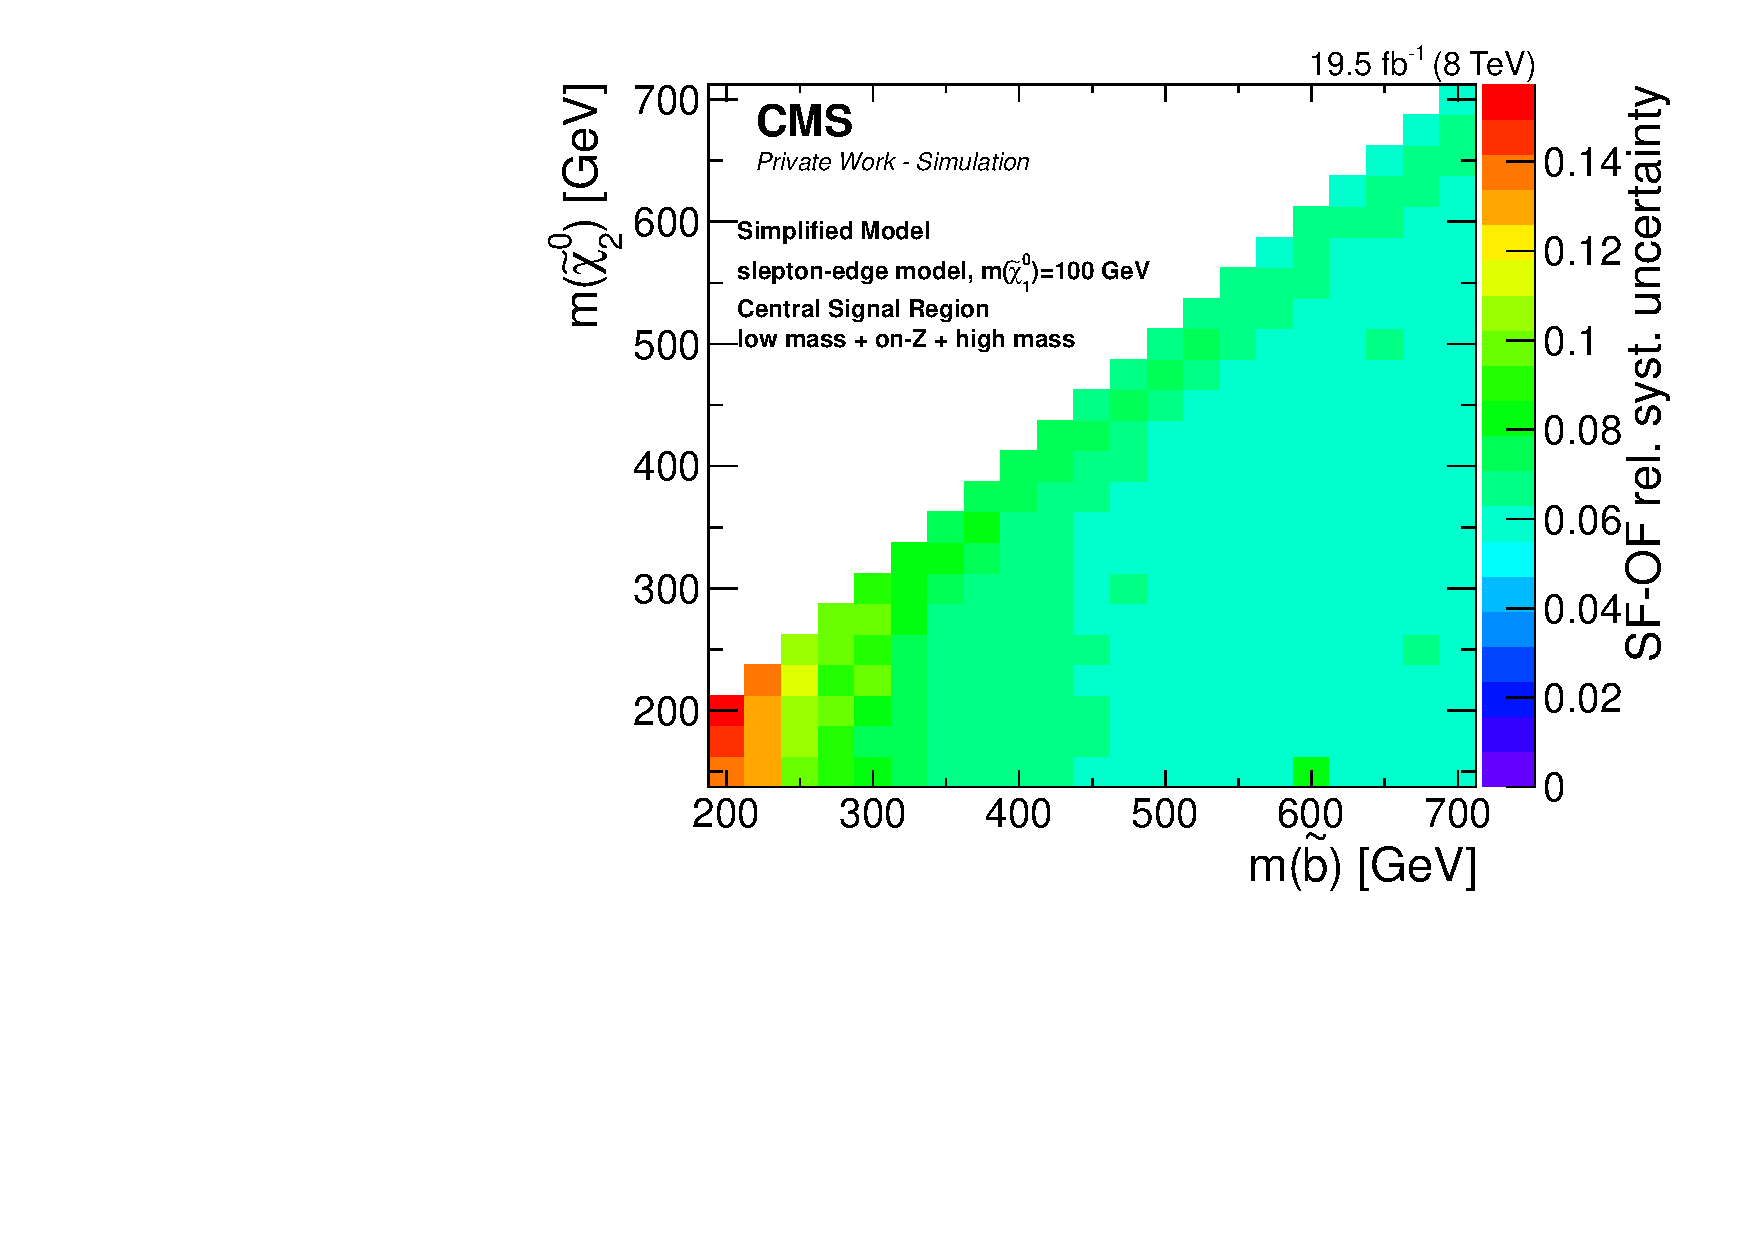
\includegraphics[width=\textwidth]{plots/limits/T6bbllslepton_m_n_1_100_Barrel_syst_err_Reweighted.pdf}
\end{minipage}
\caption{Systematic uncertainty on the signal yield in the central signal region in the $m_{\sbottom}$-$m_{\secondchi}$ plane for the fixed-edge (left) and slepton-edge (right) model.}
\label{fig:sys}
\end{figure}
\subsection{Statistical interpretation}
The results of the counting experiment are translated into exclusion limits by testing the compatibility of the signal plus background ($s+b$) and background only ($b$) hypothesis, treating each signal point in the parameter scans as a separate signal hypothesis. For this purpose, a likelihood function is defined~\cite{HiggsTool1}
\begin{equation}
\label{eq:like}
\mathcal{L}(data|\mu,\theta) = \text{Poisson}(data|\mu\cdot s(\theta) + b(\theta))\cdot p(\tilde{\theta}|\theta),
\end{equation}
where $\mu$ is a signal strength parameter, $\mu = 0$ corresponding to the background only hypothesis and $\mu > 0$ to the  $s+b$ hypothesis, and $p(\tilde{\theta}|\theta)$ parametrises the nuisance parameters $\theta$, with $\tilde{\theta}$ being the nominal value of these parameters. Based on these likelihoods, a test statistic is defined utilizing a profile likelihood ratio: 
\begin{equation}
\tilde{q_{\mu}} = -2 ln\frac{\mathcal{L}(data|\mu,\hat{\theta}_\mu)}{\mathcal{L}(data|\hat{\mu},\hat{\theta})},
\end{equation}
where the $\hat{\theta}_\mu$ represent the maximum likelihood estimators for the nuisance parameters for a given $\mu$, whereas $\hat{\mu}$ and $\hat{\theta}$ indicate the global maximum of the likelihood. For the parametrisation of the nuisance parameters $p(\tilde{\theta}|\theta)$ in equation~\ref{eq:like}, log-normal distributions are chosen. The distribution of the test statistics is then sampled dicing pseudo-experiments for some $\mu > 0$ and $\mu = 0$, representing the $s+b$ and $b$ hypotheses that are tested. The p-values $p_{s+b}$ and $p_{b}$ are defined as the probability to obtain a value of the test statistics as large or larger than the one observed in data for the given hypothesis. To obtain an upper limit on the signal cross section the value of $\mu$ is chosen where $\mathrm{CL}_{\mathrm{s}} = \frac{p_{s+b}}{p_b}$ equals 0.05, corresponding to a 95\% confidence level (CL). In the calculation, all six bins of the counting experiment are combined by multiplying the likelihoods of the different channels. In this procedure, all uncertainties on both background and signal are assumed to be uncorrelated among each other but fully correlated among the different bins.

The resulting exclusion limits are shown in Figure~\ref{fig:limits}. The left plot shows the exclusion limit in the $m_{\sbottom}$-$m_{\secondchi}$ plane for the fixed-edge model. As this model is specifically tuned to provide signals consistent with the excess observed in the low-mass central signal region, the observed limit deviates from the expected one by about $\unit{75}{\giga\electronvolt}$. Given the assumption of this model, \sbottom masses up to about $\unit{375}{\giga\electronvolt}$ are excluded, depending on the mass of the \secondchi. The right plot shows the limit for the slepton-edge model. Because of the much larger branching fraction into leptons in this model, higher masses can be excluded. The expected limit reaches \sbottom masses of about $\unit{600}{\giga\electronvolt}$ roughly independent of $m_{\secondchi}$, except for the region around $m_{\secondchi} = \unit{225}{\giga\electronvolt}$, where it drops below $\unit{550}{\giga\electronvolt}$ because of the gaps in acceptance discussed above. For lower $m_{\secondchi}$ the observed limit is significantly weaker than the expected one as here the limit is dominated by the low-mass signal region in which the excess was observed. For higher $m_{\secondchi}$, the observed limit agrees with the expected one within one standard deviation. The observed lower limit on $m_{\sbottom}$ ranges from $\unit{470}{\giga\electronvolt}$ to $\unit{590}{\giga\electronvolt}$, depending on $m_{\secondchi}$.
\begin{figure}[htbp]
\centering
\begin{minipage}[t]{0.49\textwidth}
  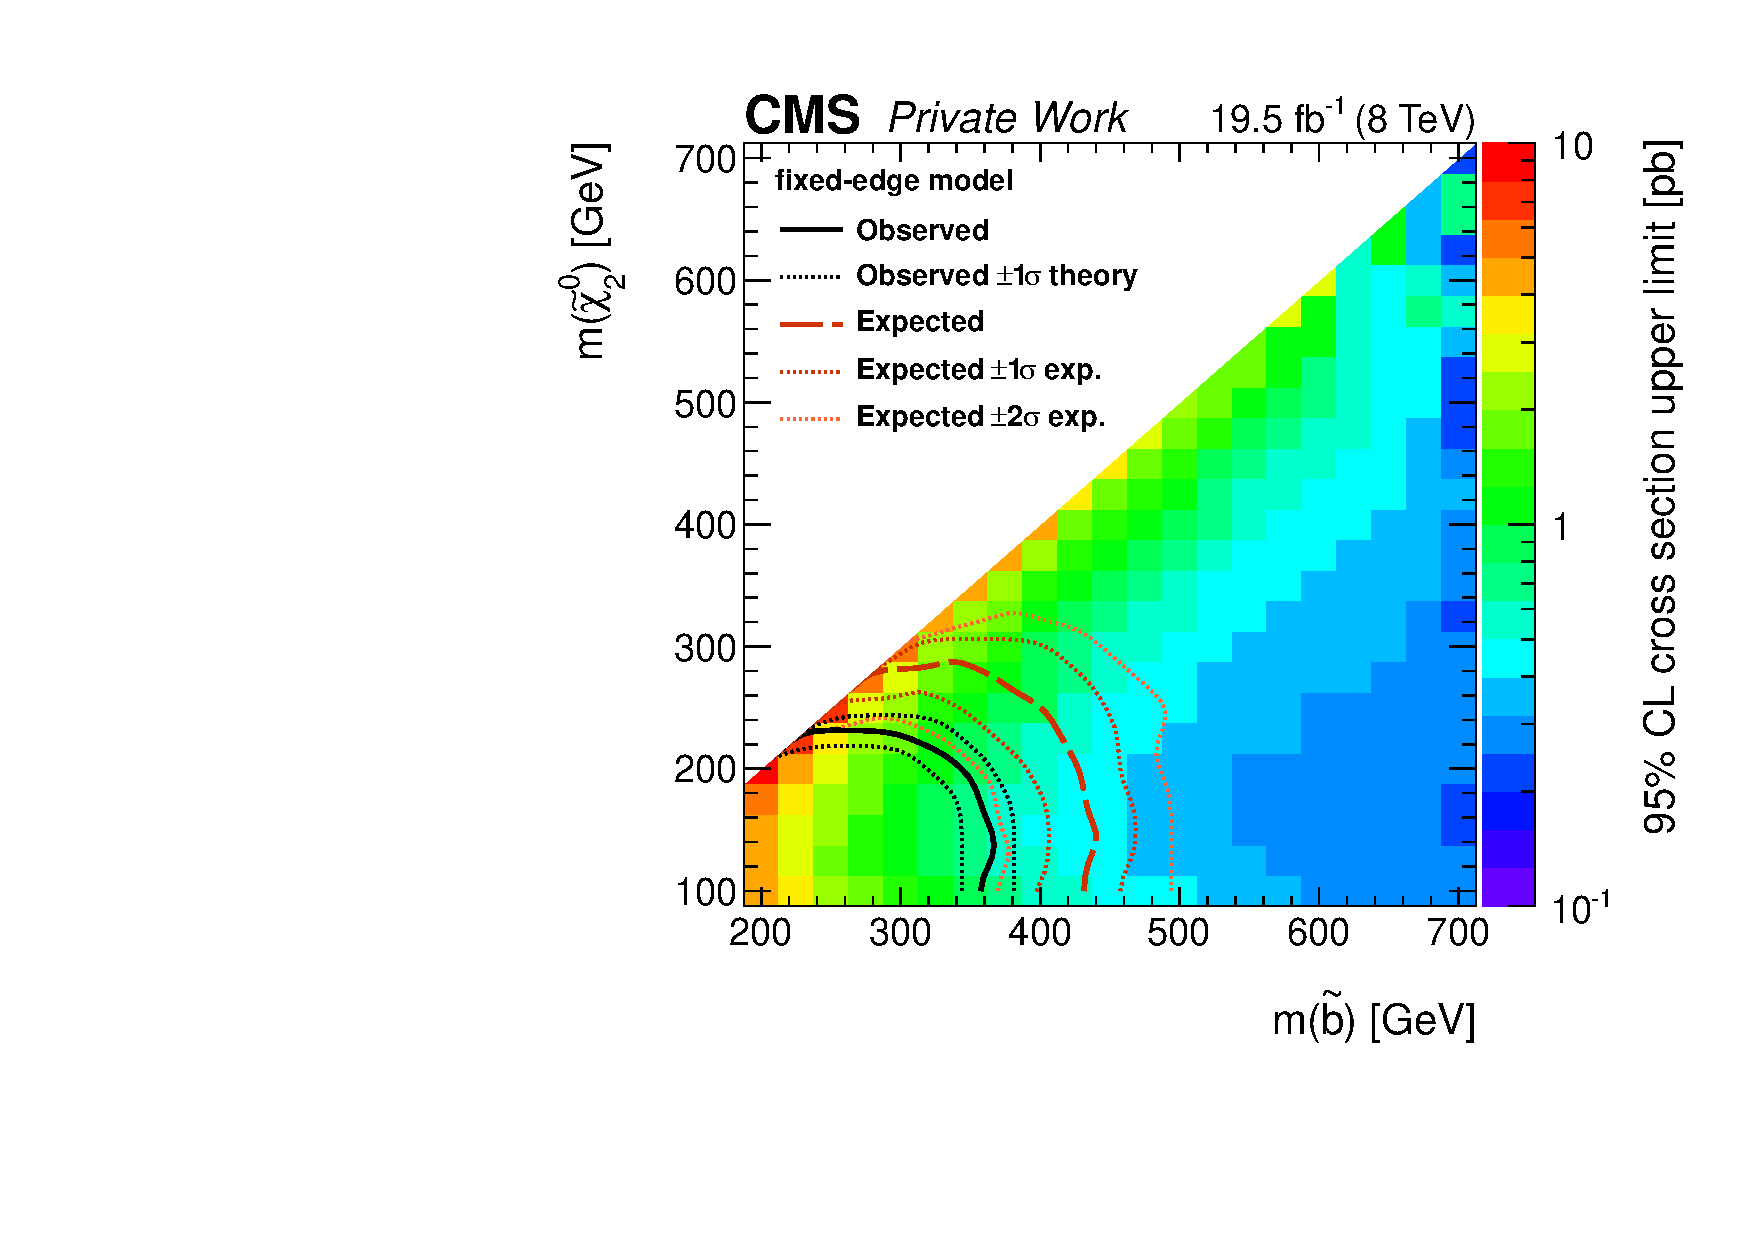
\includegraphics[width=\textwidth]{plots/limits/Fixed_Edge_sbottom_neutralino2_Exclusion_witXsecLimit.pdf}
\end{minipage}
\begin{minipage}[t]{0.49\textwidth}
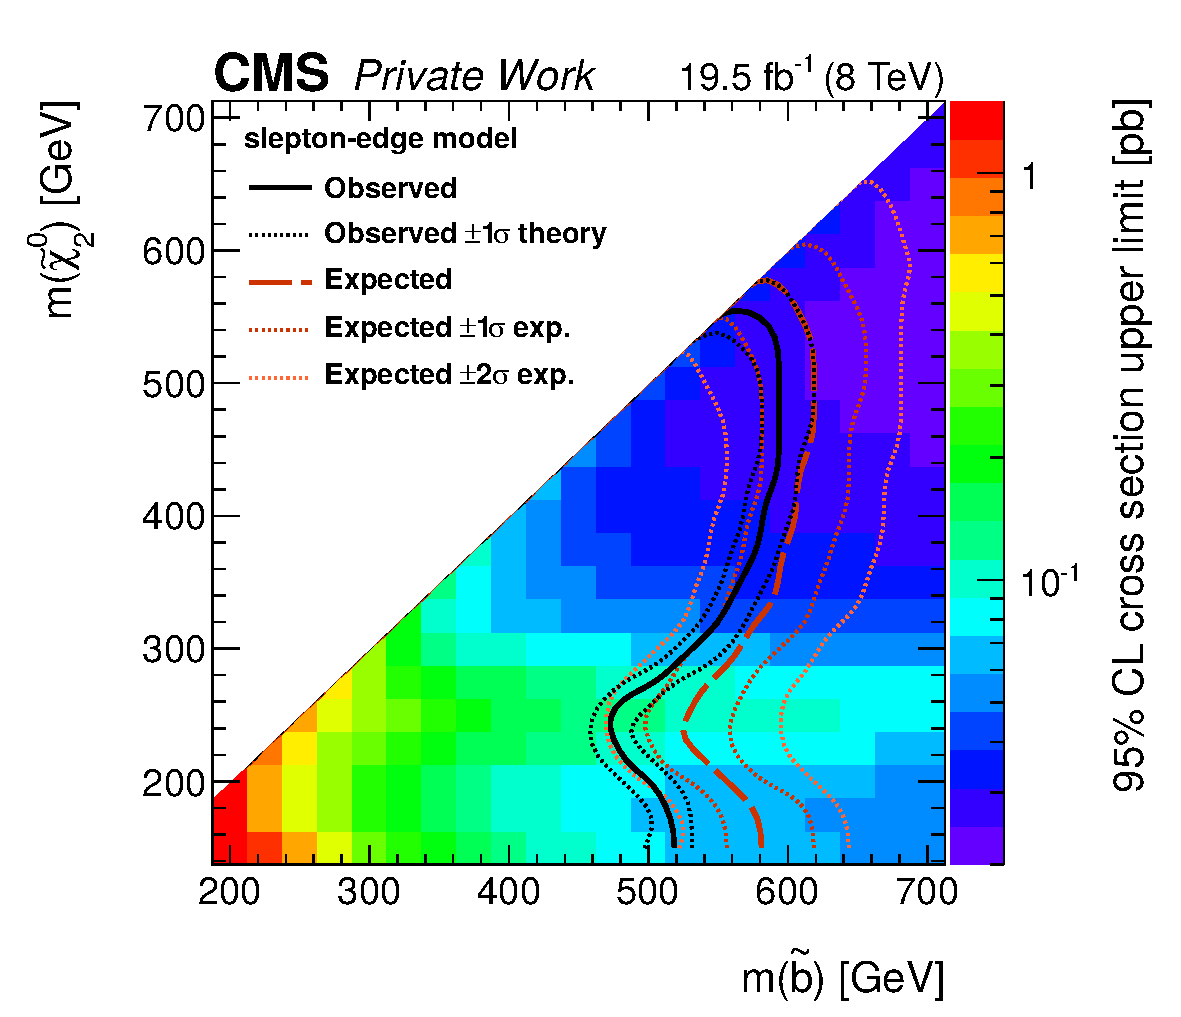
\includegraphics[width=\textwidth]{plots/limits/Fixed_Neutralino_sbottom_neutralino2_Exclusion_witXsecLimit.pdf}
\end{minipage}
\caption{Exclusion limits in the $m_{\sbottom}$-$m_{\secondchi}$ plane for the fixed-edge (left) and slepton-edge (right) model. For each signal point the upper cross section limit is shown colour coded. The intersection of the theoretical with the excluded cross section is shown as a solid black line, with every signal point to the left and below the curve being excluded. The $1-\sigma$ uncertainty interval on the observed limit is shown as dotted black lines. The expected limit together with the $1-$ and $2-\sigma$ interval are shown as brownish solid and dashed lines.}
\label{fig:limits}
\end{figure}